L'ultima tipologia di rivelatore che trattiamo sono i rivelatori a semiconduttore, detti anche rivelatori a stato solido. Questi rivelatori si basano sull'utilizzo di materiali semiconduttori, i quali sono dei materiali cristallini cioè costituiti da una struttura ordinata di atomi in un reticolo, in particolare i primi che sono stati inventati si basano sull'utilizzo di silicio o germanio.

Sono anche detti rivelatori a stato solido, perché hanno una densità che è circa mille volte maggiore rispetto a quella dei gas. Ciò costituisce una notevole differenza rispetto ai rivelatori a gas, i quali si basano sull'utilizzo di un gas a densità molto basse, mentre qui abbiamo un materiale solido e questo comporta delle differenze nelle caratteristiche che andremo ad approfondire.

\section{Semiconduttori puri}
I primi rivelatori che ormai hanno una loro storia: i primi prototipi sono stati sviluppati negli anni '60, da allora ci sono stati enormi sviluppi e oggi abbiamo rivelatori al silicio particolarmente performanti pensati per diversi tipi di applicazione, per cui in questo capitolo introdurremo il concetto di base di rivelazione basata sul semiconduttore, cioè come è stato inventato il rivelatore dal semiconduttore, per poi vedere alla fine alcune applicazioni e alcuni esempi di come i rivelatori al semiconduttore sono stati sviluppati e migliorati nel corso degli anni.

\subsection{Vantaggi e svantaggi}

I rivelatori a semiconduttore hanno diversi vantaggi:
\begin{itemize}[leftmargin=0.5cm]
   \item Hanno un'ottima risoluzione energetica.\\
   Durante il primo ciclo di esperienze è stato possibile misurare la risoluzione in energia\footnote{Ricordiamo che la risoluzione in energia esprime la capacità di un rivelatore di distinguere due valori in energia molto vicini tra di loro, per cui se la risoluzione non è buona quello che succede è che si rischia di non riuscire a distinguere due valori in energia molto vicini tra di loro.} con un rivelatore a scintillazione. In tale esperienza si hanno degli spettri acquisiti utilizzando le sorgenti $\gamma$, e andando a guardare la larghezza del picco fotoelettrico è possibile valutare la risoluzione in energia. Svolgendo tale operazione, ci si rende conto che un sistema basato sull'utilizzo di uno scintillatore e di un fotomoltiplicatore porta ad avere risoluzioni in energia che non sono particolarmente spinte, dell'ordine del 5-10\%. I rivelatori a semi-conduttore invece presentano delle buone risoluzioni energetiche;
   \item Hanno elevato stopping power.\\
   Infatti il fatto di avere a disposizione un materiale solido fa sì che la radiazione che penetra all'interno del rivelatore venga più facilmente arrestata, quindi perda più facilmente energia. Pensiamo ad esempio alla perdita di energia di un elettrone che deve entrare in un rivelatore a gas oppure in un rivelatore a silicio: nel rivelatore a silicio percorre veramente pochi millimetri, in un rivelatore a gas potrebbe percorre diversi centimetri. Quindi questo fa sì che affinché ad esempio il rivelatore venga utilizzato per misurare tutta l'energia di una particella sono sufficienti spessori e dimensioni compatte. Ad esempio in laboratorio utilizziamo questi rivelatori per misurare particelle $\alpha$ da 5 meV, le quali vengono arrestate in poche decine di micron di silicio, quindi è sufficiente un rivelatore spesso $50 \; \rm \mu m$ come quello che utilizziamo in laboratorio per essere sicuri che le particelle $\alpha$ vengano arrestate all'interno del rivelatore, quindi ne misuriamo tutta l'energia;
   \item In generale questi rivelatori, che sono sostanzialmente delle giunzioni P-N polarizzate inversamente, richiedono delle basse tensioni di alimentazione, il che costituisce un vantaggio da un punto di vista pratico.\\
   Se facciamo un confronto con i fotomoltiplicatori che richiedono centinaia di Volt, o anche con il contatore Geiger, nel quale si adoperano tensioni dell'ordine di $300-400$ Volt, per il rivelatore al silicio sono sufficienti tensioni molto più piccole, dell'ordine di decine di Volt per la polarizzazione.
   \item Hanno una risposta abbastanza veloce, cosa che invece non avevamo per i rivelatori a gas, i quali sono dei rivelatori piuttosto solenti proprio per i meccanismi e i fenomeni che avvengono al loro interno. Ciò è utile soprattutto per le misure di timing.
\end{itemize}

Tuttavia ci sono anche degli svantaggi:
\begin{itemize}[leftmargin=0.5cm]
   \item Il principale svantaggio è il fatto che questi rivelatori sono parecchio sensibili alla temperatura, quindi le condizioni di lavoro possono cambiare a seconda della temperatura in cui si sta operando. A volte alcuni di questi richiedono addirittura un sistema di raffreddamento perché altrimenti il rumore sarebbe eccessivamente elevato. \E il caso dei rivelatori al germanio, i quali necessitano di un raffreddamento;
   \item Il danneggiamento da radiazione. Infatti, essendo il semiconduttore composto da un reticolo, cioè da una struttura ordinata, quando viene sottoposto a un'elevata dose di radiazione questa dose può produrre dei danni al reticolo, quindi modificare in qualche modo la struttura ordinata del reticolo e causare delle conseguenze sul funzionamento del rivelatore. Ciò non costituisce un problema per le esperienze che svolgiamo in laboratorio dal momento che noi utilizziamo una sorgente $\alpha$ che ha un'attività abbastanza bassa. Questi problemi si presentano laddove questi rivelatori devono essere adoperati in presenza di alte radiazioni, come nel caso di esperimenti sotto fascio dunque in un acceleratore, oppure esperimenti nello spazio dove la radiazione cosmica diventa importante perché non si è più schermati dal filtro dovuto all'atmosfera terrestre;
   \item Dimensioni compatte. Tale aspetto può costituire uno svantaggio, in quanto dover rivestire una superficie molte estesa con un rivelatore a semiconduttore è estremamente costoso e anche impegnativo dal punto di vista di elettronica e del consumo, per cui quando si deve realizzare un rivelatore a semiconduttore di dimensioni estese, nascono altre problematiche e può essere non facile affrontarle.
\end{itemize}

\subsection{Banda di valenza e banda di conduzione}
Richiamiamo velocemente le proprietà dei semiconduttori.

I materiali solidi si distinguono in tre categorie diverse a seconda dello struttura a bande dei livelli di energia:
\begin{figure}[H]
   \centering
   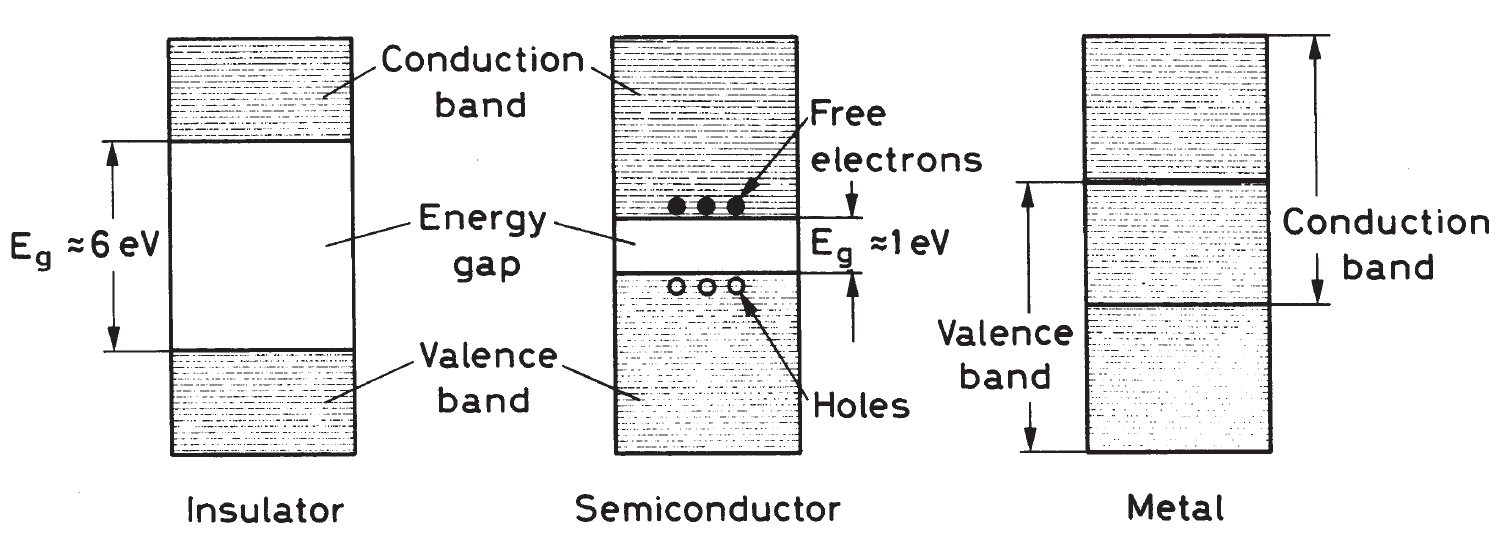
\includegraphics[width=0.9\textwidth]{immagini/bande_valenza_e_conduzione.png}
\end{figure}
In generale se banda di valenze e quella di conduzione sono separati da un gap abbastanza esteso in cui non possono essere presenti dei livelli energetici, una gap di energia proibita, abbiamo un materiale isolante, mentre il gap è inesistente abbiamo un materiale conduttore. Una situazione intermedia è quella dei materiali semiconduttori, dove questa gap è presente  però non ha una dimensione molto grande, dell'ordine di alcuni electron volt quindi esiste ma è abbastanza piccola.

Vediamo che succede se applichiamo un campo elettrico a queste tre tipologie di materiale:
\begin{itemize}[leftmargin=0.5cm]
   \item In un isolante non comporta il passaggio di corrente, perché tutti gli elettroni si trovano nella banda di valenza e quindi non abbiano conduzione;
   \item In un conduttore si osserva il passaggio di una corrente;
   \item In un semiconduttore si osserva una piccolissima corrente legata al fatto che alcuni elettroni, che definiamo elettroni termici i quali hanno acquisito un'energia per effetti termici sufficiente a superare il gap energetico, possono condurre. \E chiaro che è un effetto puramente statistico, dovuto all'agitazione termica, quindi si genera una corrente abbastanza debole.
\end{itemize}
Nei semiconduttori abbiamo un'altra caratteristica fondamentale, cioè il fatto che i portatori di carica, cioè le cariche che generano una corrente possono essere di due tipologie, \textit{elettroni} e \textit{lacune}.
\begin{figure}[H]
   \centering
   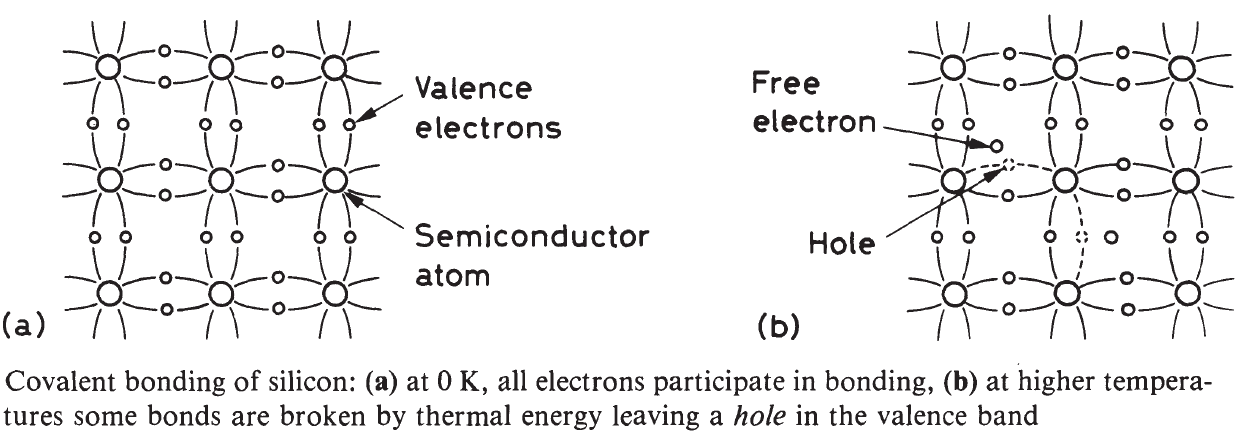
\includegraphics[width=0.9\textwidth]{immagini/elettroni_e_lacune_semiconduttori.png}
\end{figure}
Le lacune sono delle vacanze di elettroni e anch'esse concorrono al valore della corrente in un semiconduttore, quindi ogni volta che noi andremo a parlare di questi effetti di corrente, faremo riferimento sia elettroni che lacune.

\subsection{Creazione di coppie}

Normalmente, in un semiconduttore esistono due fenomeni che sono in competizione l'uno con l'altro:

\begin{enumerate}[leftmargin=0.6cm]
   \item Creazione di coppie elettrone-lacuna che abbiamo già accennato, cioè per effetti termici effettivamente un elettrone potrebbe passare dalla banda di valenza alla banda di conduzione e quindi si viene a creare una coppia elettrone-lacuna;
   \item Ricombinazione, cioè un elettrone potrebbe ricombinarsi con una lacuna, purché i valori di energia e di impulso lo consentono.
\end{enumerate}

Analizziamo il primo fenomeno. \E chiaro che in generale, in un semiconduttore puro, detto anche intrinseco\footnote{Da non confondere con il semiconduttore intrinseco visto negli APD.}, il numero di elettroni che si trova nella banda di conduzione è esattamente uguale al numero delle lacune in banda di valenza, perché ogni volta che un elettrone viene promosso salta dalla banda di valenza alla banda di conduzione e crea la sua lacuna corrispondente. Sia gli elettroni che le lacune contribuiscono alla conducibilità elettrica del semiconduttore. 

Cerchiamo allora di capire quanto vale la concentrazione di elettroni e di lacune. Dal momento che stiamo considerando un semiconduttore puro, il numero di elettroni corrisponde al numero di lacune, dunque indichiamo la concentrazione in generale con $n_i$, che sarà data da
\begin{equation*}
   n_i
   =\sqrt{N_C N_V} \exp{ -\frac{E_g}{2k_B T} }
   =AT^{\frac{3}{2}} \exp{ -\frac{E_g}{2k_B T} }
\end{equation*}
dove
\begin{itemize}[leftmargin=0.5cm]
   \item $N_C$ e $N_v$ sono rispettivamente il numero di possibili stati nella banda di conduzione e in quella di valenza;
   \item $E_g$ è l'energia della gap proibita;
   \item $T$ è la temperatura;
   \item $k_B$ è la costante di Boltzmann
   \item $A$ è una costante indipendente dalla temperatura
\end{itemize}

Le dipendenze dall'energia della gap e dalla temperatura nell'esponenziale decrescente sono abbastanza intuitive: per quanto riguarda $E_g$, se la gap è piccola per un elettrone sarà più facile lasciare la banda di valenza e andare verso la banda di conduzione, viceversa più è elevata la temperatura più sarà probabile che un elettrone possa passare alla banda di conduzione per effetto termico, ecco perché lo si trova al denominatore. Utilizzando la statistica di Fermi-Dirac, è possibile inoltre valutare il numero di stati nella banda di conduzione e dalla banda di valenza. Si trova che il loro prodotto è pari a $N_C N_V=AT^3$. In definitiva, la concentrazione di elettroni e lacune libere dovuto soltanto all'effetto termico dipende dalle caratteristiche del semiconduttore (in particolare da $E_g$) e dalla temperatura $T$. 

Vediamo quanti elettroni e lacune abbiamo a temperatura ambiente per due semiconduttori, silicio e germanio, i quali si differiscono per le dimensioni della gap. Supposto di avere una temperatura di 300 K, troviamo una concentrazione di $2.5 \cdot 10^{13}/\rm cm^3$ per il germanio e $1.5 \cdot 10^{10}/\rm cm^3$ per il silicio. Se consideriamo che in media abbiamo $10^{22} \text{ atomi/cm}^3$, tali valori corrispondono rispettivamente a dire che soltanto un elettrone su $10^9$ atomi per il germanio un elettrone su $10^{12}$ atomi per il silicio si trova nella banda di conduzione, quindi effettivamente non sono tantissimi. Ciò ha una corrispondenza con quanto affermato prima, ossia che se applichiamo un campo elettrico a un materiale semiconduttore si genera una corrente molto piccola, ed effettivamente è così perché troviamo poche coppie elettrone-lacune dovute ad effetti termici.
\subsection{mobilità}
Sotto l'azione di un campo elettrico $E$, elettroni e lacune cominciano a muoversi, cioè subiscono un moto di deriva. Possiamo valutare le velocità con cui avviene questa deriva: esse sono date da\footnote{Il pedice $h$ sta per "hole", cioè lacuna in inglese.}
\begin{equation*}
   v_e=\mu_e E
   \qq{,}
   v_h=\mu_h E
\end{equation*}
Come possiamo vedere, le velocità di elettroni e lacune sono proporzionali al valore del campo elettrico e alla mobilità, che sono diverse per elettroni e lacune. Queste mobilità non sono costanti, dipendono dal valore del campo elettrico e della temperatura, ad esempio per il silicio a temperature normali troviamo che le mobilità $\mu_e$ e $\mu_h$:
\begin{itemize}[leftmargin=0.5cm]
   \item risultano essere costanti per valori di campo elettrico inferiori a $10^3 \; \rm V/cm$;
   \item hanno una dipende del tipo $E^{-\frac{1}{2}}$ per valori di campo elettrico compresi tra $10^3-10^4 \; \rm V/cm$;
   \item hanno una dipende del tipo $E^{-1}$ per valori di campo maggiori di $10^4 \; \rm V/cm$.
\end{itemize}
Tale andamento ha come conseguenza il fatto che arrivati a un certo punto si giunge a una saturazione della velocità a un valore massimo di $10^7$ cm/s, legato al fatto che l'energia che viene acquisita da questi elettroni e queste lacune viene poi persa per gli urti con il reticolo.

Alla luce di quanto visto, la conduttività di un semiconduttore si può esprimere considerando sia il contributo dovuto agli elettroni che quello dovuto alle lacune:
\begin{equation*}
   \sigma=e n_i (\mu_e + \mu_h)
\end{equation*}
\subsection{Ricombinazione e trapping}

Può avvenire una ricombinazione spontanea, cioè legata al fatto che elettrone e lacune aventi opportuni valori di energia ed impulso possono ricombinarsi e dare luogo all'emissione di un fotone. Tale processo è un meccanismo raro, perché non è sufficiente che elettroni e lacune si trovino vicine per ricombinarsi, ma devono avere anche dei valori opportuni di energia e impulso. A riprova della sua rarità, la vita media di una coppia che è stata creata per effetti termici è dell'ordine di un secondo, dopodiché per qualche motivo c'è una ricombinazione e tale coppia cessa di esistere. Sebbene un secondo possa sembrare un tempo piccolo, se confrontato con i tempi caratteristici dei rivelatori risulta essere un tempo enorme, dunque questa coppia sopravvive parecchio.

Tuttavia quello che si osserva sperimentalmente è che la vita media di una coppia è molto più bassa di un secondo, quindi evidentemente ci sono altri meccanismi oltre alla ricombinazione spontanea che portano alla scomparsa della coppia. Questi meccanismi sono legati alla presenza dei centri di ricombinazione.

\begin{figure}[H]
   \centering
   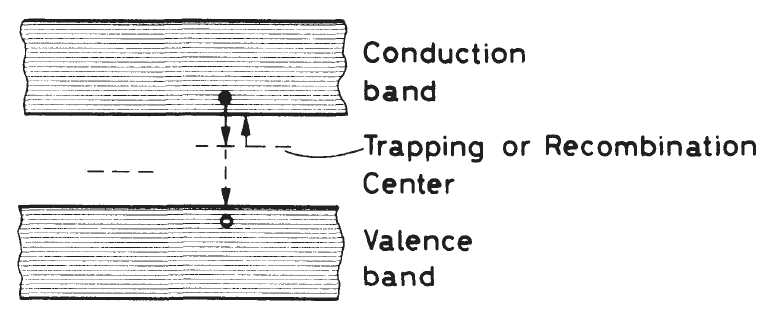
\includegraphics[width=0.55\textwidth]{immagini/centri_di_ricombinazione.png}
\end{figure}

Infatti, a causa di difetti della struttura cristallina si possono presentare dei livelli nella zona proibita, i quali sono dei livelli che vengono definiti profondi nel senso che sono abbastanza distanziati sia dalla banda di conduzione che dalla banda di valenza (lo possiamo vedere tratteggiati in figura). In questi livelli si può verificare una ricombinazione perché sono livelli che possono attrarre elettroni dalla banda di conduzione e lacune della banda di valenza permettendo quindi una ricombinazione. Ecco perché vengono definiti come centri di ricombinazione.

Tali centri di ricombinazione fanno sì che alla fine la vita media di una coppia sia effettivamente più bassa.

\vspace{0.2cm}Da un punto di vista della rivelazione, visto che il rivelatore a semiconduttore produce per effetto del passaggio di una particella coppie elettrone-lacuna su cui si basa il segnale, ci interessa che tali coppie non si ricombinino prima di riuscire a raccoglierle, dunque non vogliamo che la vita media sia eccessivamente bassa perché se queste coppie si ricombinano troppo rapidamente perdiamo il segnale. In conseguenza a ciò i semiconduttori che adoperiamo nei rivelatori devono essere estremamente puri, cioè devono presentare pochi difetti perché più difetti ci sono più aumentano i centri di ricombinazione.

Alcuni centri di ricombinazione sono anche definiti dei centri trappola. Sono dei livelli dove viene catturata soltanto una tipologia di carica, quindi ad esempio viene catturato un elettrone dalla banda di conduzione e l'elettrone rimane in tale sito per parecchio tempo, da cui il nome livelli trappola.

\vspace{0.2cm}Vediamo ora che tipo di difetti possono essere presenti in un reticolo cristallino come quello di un semiconduttore
\begin{figure}[H]
   \centering
   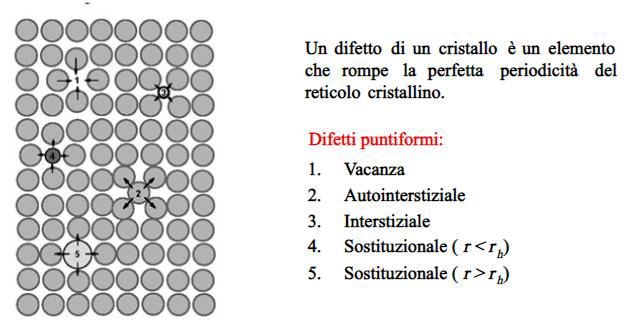
\includegraphics[width=0.7\textwidth]{immagini/difetti_cristallini.png}
\end{figure}
In questa figura sono rappresentate i principali difetti di un reticolo:
\begin{itemize}[leftmargin=0.5cm]
   \item Potremmo avere una vacanza, cioè l'assenza di un atomo che era previsto nel reticolo;
   \item Potremmo avere un difetto è autointerstiziale, che è l'opposto della vacanza, in quanto si ha un atomo dello stesso tipo del cristallo in più rispetto a quanto previsto dello schema del reticolo;
   \item Potremmo avere un difetto interstiziale, che si differenze dal precedente per il fatto che abbiamo sempre un atomo in più rispetto a quanto previsto però è un atomo di natura diversa;
   \item Potremmo infine avere dei difetti sostituzionali, cioè un atomo del semiconduttore viene sostituito con un atomo di tipologia diversa, però affinché ciò avvenga le dimensioni devono essere abbastanza simili, dunque i raggi dei due automi devono essere similari.
\end{itemize}
Ogni difetto del reticolo comporta una modifica nello schema dei livelli energetici. Scegliendo però in maniera opportuna degli elementi da aggiungere al reticolo cristallino, ossia con opportuni drogaggi, possiamo generare degli ulteriori livelli energetici superficiali, ossia livelli che sono vicini o alla banda di conduzione o alla banda di valenza. Per questo motivo nella pratica si utilizzano semiconduttori drogati.

\section{Semiconduttori drogati}
In un semiconduttore drogato, detto anche semiconduttore estrinseco, si vanno a sostituire gli atomi del semiconduttore con atomi di elementi diversi. Ad esempio, caso di silicio e germanio, i quali sono entrambi tetravalenti cioè hanno quattro elettroni di valenza, per drogarli è necessario introdurre atomi trivalenti o atomi pentavalenti.

La conseguenza del drogaggio è una variazione nella proporzione tra elettroni e lacune. Infatti in un semiconduttore puro il numero di elettroni coincide con il numero delle lacune generati per effetti termici, mentre drogando il materiale creiamo uno squilibrio.

\subsection{Semiconduttori di tipo n}
In un semiconduttore drogato di tipo n si va a sostituire un atomo del reticolo con un atomo pentavalente, come ad esempio l'arsenico, il fosforo o l'antimonio.
\begin{figure}[H]
   \centering
   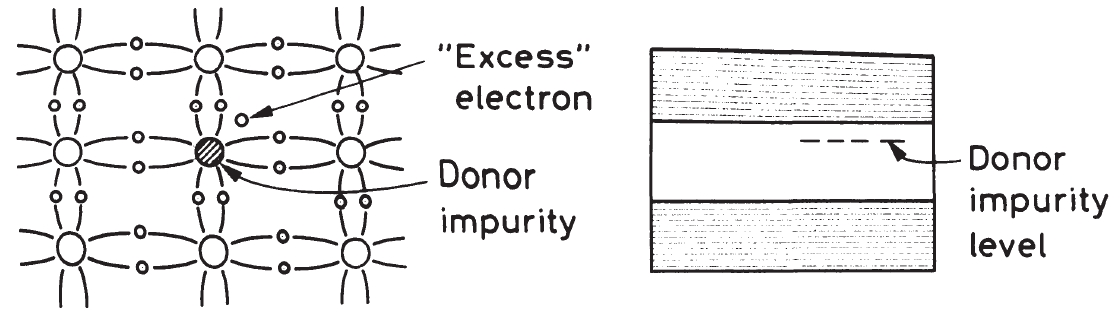
\includegraphics[width=0.8\textwidth]{immagini/semiconduttori_drogati_tipo_n.png}
\end{figure}
Questo atomo avrà 5 elettroni di cui 4 vanno a legarsi con i quattro atomi di silicio che si trovano attorno, mentre il quinto elettrone rimane in eccesso e può essere un elettrone di conduzione. L'aggiunta di un tale atomo corrisponde a generare nella zona del gap proibito di energie un livello superficiale, che in questo caso è molto vicino alla banda di conduzione, a una distanza di 0,01 eV nel caso del Germania o 0,05 eV nel caso del silicio. Questo elettrone si troverà in questo livello discreto, per cui gli sarà sufficiente una piccolissima energia per essere in grado di passare alla banda di conduzione, quindi sostanzialmente è un elettrone quasi libero.

Con valori di drogaggio tipici si può raggiungere un numero di elettroni di conduzione di $10^{17}\text{ elettroni/cm}^3$, mentre il numero di lacune si riduce a $10^3\text{ lacune/cm}^3$. Ecco perché nei semiconduttori drogati di tipo n i portatori di carica maggioritari sono gli elettroni mentre le lacune rappresentano i portatori di carica minoritari.
\subsection{Semiconduttori di tipo p}
La situazione è diametralmente opposta in semiconduttore drogato di tipo p. In questo caso si va a sostituire un atomo del reticolo con un atomo trivalente come il gallio, il borro o l'indio e quello che stavolta rimane in eccesso è una lacuna.
\begin{figure}[H]
   \centering
   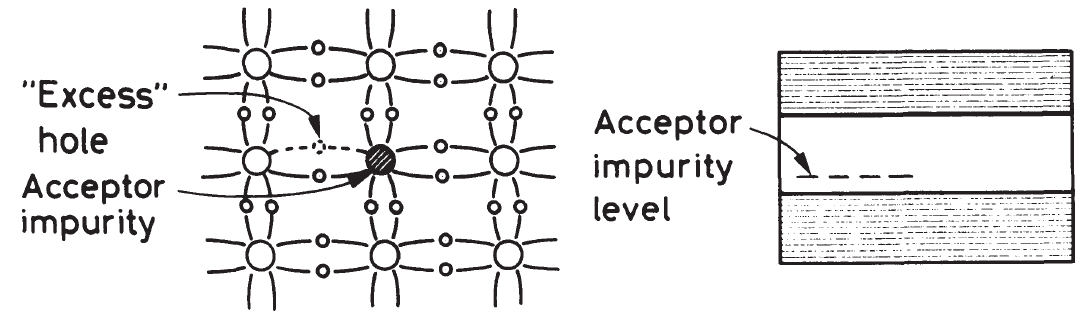
\includegraphics[width=0.8\textwidth]{immagini/semiconduttori_drogati_tipo_p.png}
\end{figure}

Questa lacuna si troverà in un livello discreto situato nella banda di energia probita, a una distanza molto piccola dalla banda di valenza. In questo caso le lacune rappresentano i portatori di carica maggioritari e gli elettroni quelli minoritari.

Va precisato che anche se introduciamo un'impurezza ossia un atomo di tipo diverso, il materiale rimane comunque neutro. Infatti nel caso in cui ad esempio introduciamo un'impurità di tipo n cioè un donore, sebbene ci sia un elettrone in eccesso ciò non vuol dire che il materiale è carico negativamente, perché abbiamo la carica del nucleo che compensa l'elettrone libero. ne segue che complessivamente abbiamo un materiale neutro. Analoghi ragionamenti valgono nel caso in cui introduciamo un atomo accettore.

\subsection{Concentrazione di elettroni e lacune}
Si può dimostrare che, indipendentemente del tipo di drogaggio, il prodotto della concentrazione di elettroni $n$ per la concentrazione di lacune $p$ è sempre data da
\begin{equation*}
   np=n_i^2
\end{equation*}
dove $n_i$ è la concentrazione nel caso del semiconduttore intrinseco.

Da tale relazione segue che se aumentano gli elettroni per effetto di un drogaggio, la quantità delle lacune che si formano nel semiconduttore non rimane costante ma diminuisce e viceversa nel caso opposto. 

La legge appena enunciata prende il nome di legge dell'azione di massa. Partendo da tale legge, in un semiconduttore di tipo n, dove ci aspettiamo che il numero di atomi accettori $N_A$ sia pari a zero mentre il numero di atomi donori $N_D$ comporti la formazione di un medesimo numero di elettroni\footnote{Gli atomi accettori e donori sono rispettivamente elementi che accettano elettroni e donano elettroni dal/al semiconduttore.}, possiamo esprimere la concentrazione di lacune e la conducibilità del materiale come segue:
\begin{equation*}
   p \approx \frac{n_i^2}{N_D}
   \qq{e}
   \sigma \approx e N_D \mu_e
\end{equation*}
Analogamente, per un simiconduttore drogato di tipo p, dove stavolta abbiamo $N_D=0$ e $N_A$ lacune, abbiamo 
\begin{equation*}
   n \approx \frac{n_i^2}{N_A}
   \qq{e}
   \sigma \approx e N_A \mu_h
\end{equation*}
Vediamo come a differenza di prima, dove la conducibilità veniva espressa come somma di due termini, uno dovuto agli elettroni e uno dovuto alle lacune, nel caso di semiconduttori drogati la conduzione elettrica è affidata ai portatori maggioritari di carica, ossia gli elettroni nel caso dei simiconduttori drogati di tipo N e le lacune nei casi semiconduttori drogati di tipo P. Se allora vogliamo avere una corrente più elevata, quello che dovete fare è drogare maggiormente il materiale, per cui se ad esempio abbiamo un drogaggio di tipo n dobbiamo aumentare la concentrazione degli atomi donori; viceversa nel simiconduttore di tipo p dobbiamo aumentare la concentrazione di atomi acettori.

\subsection[Semiconduttori di tipo \texorpdfstring{$\rm p+$}{p+}, \texorpdfstring{$\rm p-$}{p-}, i (compensati)]
{Semiconduttori di tipo $\boldsymbol{\rm p+}$, $\boldsymbol{\rm p-}$, i (compensati)}
Può essere utile drogare i semiconduttori con elevate concentrazioni, anche dell'ordine di $10^{20}\text{ atomi/cm}^3$ anziché i soliti $10^{13}\text{ atomi/cm}^3$. Per quanto detto prima, questi materiali risultano essere altamente conduttivi. Inoltre essi sono indicati con il simbolo "$+$" proprio per indicare che la concentrazione è elevata e vengono tipicamente adoperati per la realizzazione dei contatti elettrici. Infatti in qualsiasi rivelatore per poter estrarre un segnale elettrico abbiamo bisogno di contatti elettrici, ad esempio nel caso del rivelatore a gas abbiamo anodo e catodo da cui possiamo prelevare un segnale. Qui il materiale semiconduttore non ha dei contatti, dunque bisogna crearli, sebbene ciò non sia facile crearli perché nel momento in cui proviamo a utilizzare un materiale metallico a contatto con un semiconduttore purtroppo introduciamo degli effetti collaterali. Per evitare ciò, quello che si fa è realizzare delle zone ad alto drogaggio proprio là dove vogliamo creare il contatto ohmico con un metallo.

Per quanto riguarda i semiconduttori etichettati con la lettere "i", ingenuamente potremmo pensare che stia per intrinseco, ma in realtà non è esattamente così. Infatti un materiale di tipo i si comporta come un materiale intrinseco cioè un materiale puro, ma in realtà prende il nome di materiale compensato, perché è comunque un semiconduttore che è stato drogato, sia di tipo n che di tipo p, con la stessa concentrazione. L'effetto risultante di tale drogaggio è dunque quello di riportare il semiconduttore alla condizione di intrinseco, ma bisogna sempre ricordare che è stato drogato. Sono materiali che hanno una resistività elevata.

\subsection{Giunzioni n-p}
Il principio di base di un rivelatore a semiconduttore sono le giunzioni p-n o n-p. Se prendiamo due materiali, uno drogato di tipo n e uno drogato di tipo p, e li accostiamo uno vicino all'altro, avvengono dei fenomeni. 
\begin{figure}[H]
   \centering
   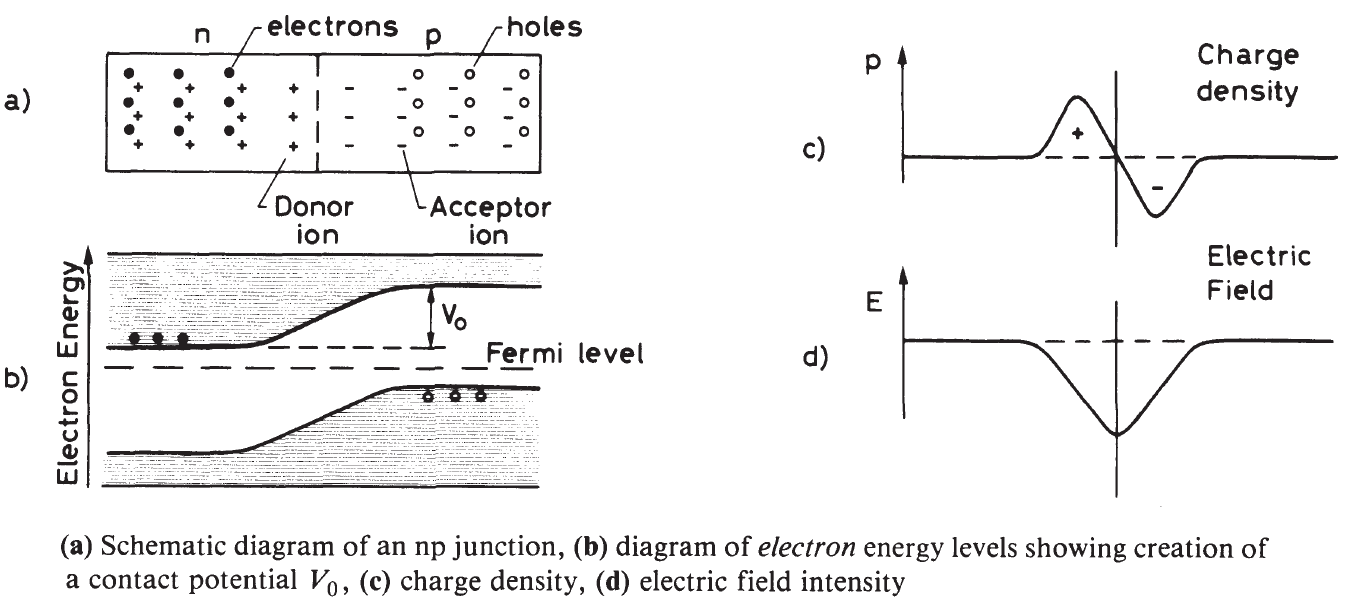
\includegraphics[width=0.8\textwidth]{immagini/giunzione_p-n.png}
\end{figure}
Poiché stiamo mettendo a contatto dei materiali che hanno concentrazione di carica diverse l'uno dall'altro (nel materiale di tipo n c'è un'elevata concentrazione di elettroni liberi, mentre nel materiale di tipo p c'è un'elevata concentrazione di lacune), si verifica una diffusione di elettroni verso il materiale di tipo p e di lacune verso il materiale di tipo n, proprio a causa di questa differente concentrazione. Gli elettroni che si diffondono nella zona di tipo p incontrano le lacune e si ricombinano con queste; lo stesso avviene nel materiale di tipo n, dove le lacune che si sono diffuse in esso si ricombinano con gli elettroni. Essendo entrambe le zone n e p inizialmente neutre, nella giunzione la zona n avrà una concentrazione di cariche positive mentre la zona p di cariche negative. Come possiamo infatti vedere dalla figura a), inizialmente in n erano presenti gli elettroni liberi mentre in n le lacune, e una volta realizzata la giunzione gli elettroni sono passati da n a p e si sono ricombinati con le lacune. In conseguenza a ciò, nella regione p sono rimasti degli ioni negativi, fissi nel reticolo. viceversa nella zona di tipo n, le lacune si sono ricombinate con gli elettroni e quindi sono rimasti fissi nel reticolo gli ioni positivi. Ciò comporta la formazione di un campo elettrico e dunque di un potenziale $V_0$, detto potenziale di contatto, che come possiamo vedere nella figura b), dove sull'asse verticale sono riportati i livelli in energia mentre l'asse orizzontale la posizione in corrispondenza con la figura a), ha deformato i livelli energetici. In altri termini, a causa della presenza di queste cariche fisse nel reticolo dei materiali di tipo p e di tipo n, si è creata una differenza di potenziale che impedisce l'ulteriore passaggio e diffusione di cariche libere. Si è allora creata una regione che dal punto di vista della rivelazione è ottimale, perché è una regione in cui non sta circolando carica libera e quindi se per caso dovesse passare una particella, la quale comporta la formazione di nuove cariche, quest'ultime possono essere spazzate via da questo potenziale e raccolte.

Il potenziale di contatto $V_0$ è abbastanza piccolo, circa $1 \; \rm V$. Inoltre la zona che si è venuta a creare prende il nome di zona di svuotamento, perché è una zona dove abbiamo eliminato tutte le cariche libere. Sono quindi presenti delle cariche fisse, che determinano un campo elettrico, ma non sono presenti cariche libere che potrebbero rappresentare rumore per i nostri scopi, in quanto sono cariche che non sono dettate dal passaggio di una radiazione, ma sono cariche che erano presenti nel materiale semiconduttore. Non essendo presenti in questa regione, essa risulta essere una regione utile per la rivelazione.

Cerchiamo allora di valutare l'estensione di tale regione. Per fare ciò consideriamo la concentrazione degli atomi accettori e degli atomi donori\footnote{La dimostrazione che segue è stata aggiunta dall'autore, la professoressa riporta soltanto i risultati finali. Si è preferito operare il tal modo piuttosto che dedicare un approfondimento a parte per non rendere ridondante la trattazione}.
\begin{figure}[H]
   \centering
   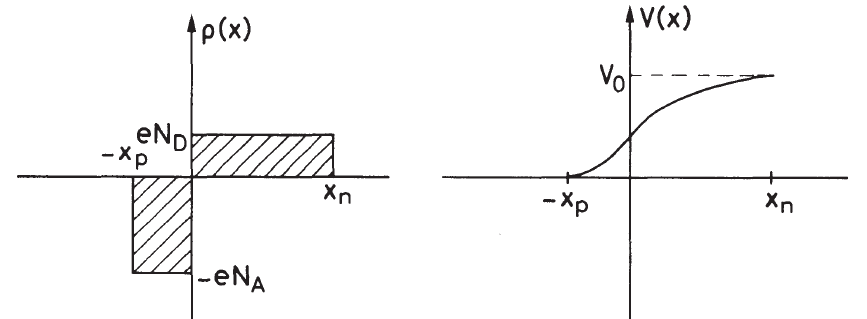
\includegraphics[width=0.8\textwidth]{immagini/modello_regione_svuotamento.png}
\end{figure}
Supponiamo di avere una distribuzione uniforme di carica attorno alla giunzione. Detta $x_n$ l'estensione della zona di svuotamento nel tipo n e $x_p$ quella nel tipo p, abbiamo:
\begin{equation*}
   \rho(x)=
   \begin{cases}
      eN_D & \text{per } 0 < x < x_n\\
      -eN_A & \text{per } -x_p < x < 0\\
   \end{cases}
\end{equation*}
dove $e$ è la carica dell'elettrone e $N_D$ e $N_A$ sono le concentrazioni di impurità donatrici e accettrici. Poiché la carica totale è conservata, abbiamo anche la relazione:
\begin{equation*}
   N_A x_p= N_D x_n
\end{equation*}
Conoscendo la densità di carica, possiamo calcolare l'ampiezza della regione di svuotamento a partire dall'equazione di Poisson:
\begin{equation*}
   \dv[2]{V}{x}=-\frac{\rho(x)}{\varepsilon}
\end{equation*}
dove $\varepsilon$ è la costante dielettrica del mezzo. Integrando una volta tale equazione troviamo:
\begin{equation*}
   \dv{V}{x}=
   \begin{dcases}
      -\frac{eN_D}{\varepsilon} x + C_n & \text{per } 0 < x < x_n\\
      \frac{eN_A}{\varepsilon} x + C_p & \text{per } -x_p < x < 0\\
   \end{dcases}
\end{equation*}
dove $C_n$ e $C_p$ sono costanti di integrazione.

Applichiamo le condizioni al contorno, secondo le quali il campo elettrico $E=-\dv*{V}{x}$ deve annullarsi su entrambi i bordi della distribuzione di carica: imponendo quindi che $\dv*{V}{x}=0$ per $x=x_n$ e per $x=-x_p$, l'equazione appena scritta diventa:
\begin{equation*}
   \dv{V}{x}=
   \begin{dcases}
      -\frac{eN_D}{\varepsilon} (x - x_n) & \text{per } 0 < x < x_n\\
      \frac{eN_A}{\varepsilon} (x + x_p) & \text{per } -x_p < x < 0\\
   \end{dcases}
\end{equation*}
Tale equazione rappresenta il campo elettrico nella regione di carica spaziale. Un'ulteriore integrazione ci fornisce:
\begin{equation*}
   V(x)=
   \begin{dcases}
      -\frac{eN_D}{\varepsilon} \qty( \frac{x^2}{2} - x_n x ) + C & \text{per } 0 < x < x_n\\
      \frac{eN_A}{\varepsilon} \qty( \frac{x^2}{2} + x_p x) + C' & \text{per } -x_p < x < 0\\
   \end{dcases}
\end{equation*}
Poiché le due soluzioni devono coincidere per $x=0$, è chiaro che $C=C'$. Inoltre per $x=x_n$ abbiamo che $V(x_n)=V_0$ che è il potenziale di contatto, quindi:
\begin{equation*}
   V_0=\frac{eN_D}{2\varepsilon} x_n^2 + C
\end{equation*}
Analogamente, sul lato p, abbiamo che $V=0$ per $x=-x_p$, quindi:
\begin{equation*}
   0=-\frac{eN_A}{2\varepsilon} x_p^2 + C
\end{equation*}
Eliminando $C$ otteniamo:
\begin{equation*}
   V_0=\frac{e}{2\varepsilon} \bigl( N_D x_n^2 + N_A x_p^2 \bigr)
\end{equation*}
Utilizzando la conservazione della carica si ottiene infine
\begin{equation*}
   x_n=\qty[ \frac{2\varepsilon V_0}{e N_D (1 + N_D/N_A)} ]^{\frac{1}{2}}
   \qq{,}
   x_p=\qty[ \frac{2\varepsilon V_0}{e N_A (1 + N_A/N_D)} ]^{\frac{1}{2}}
\end{equation*}
Vediamo come $x_n$ e $x_p$ dipendono dal potenziale di contatto $V_0$ e dalle concentrazioni.

Possiamo vedere che, se un lato è più drogato dell'altro, cosa che avviene solitamente, allora la zona di svuotamento si estenderà maggiormente nel lato meno drogato. Ad esempio, se il materiale p è più drogato rispetto a quello n, dunque se $N_A \gg N_D$, allora $x_n \gg x_p$, il che significa che la regione di svuotamento si trova quasi interamente sul lato n della giunzione.

In ogni caso le regioni di svuotamento hanno dimensioni molto piccole, tipicamente dell'ordine di $100 \; \rm \mu m$. In queste condizioni, un rivelatore basato su una giunzione p-n avrà prestazioni abbastanza limitate in termini di rumore, risoluzione e stopping power. Per migliorarlo possiamo ampliare la regione di svuotamento e ciò si fa polarizzando la giunzione, cioè applicando una differenza di potenziale esterna per aumentare la regione in cui si verifica lo svuotamento.
\begin{figure}[H]
   \centering
   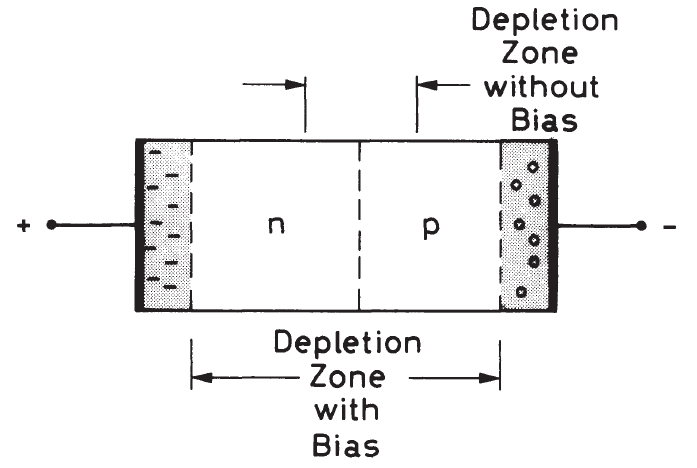
\includegraphics[width=0.6\textwidth]{immagini/regione_svuotamento_ampliata.png}
\end{figure}
Tale procedura è detta polarizzazione inversa, in quanto il potenziale positivo viene applicato al materiale di tipo n e quello negativo al materiale di tipo p.\footnote{Se la giunzione venisse polarizzata direttamente la regione di svuotamento si contrarrebbe e si avrebbe conduzione.}. In questo modo si allarga la zona di svuotamento fino a valori dell'ordine del millimetro, la quale rappresenterà il volume sensibile per la rivelazione delle particelle. Tuttavia non si può andare oltre un certo valore perché abbiamo un limite dettato dalla resistività del materiale.

\vfill

\section{Rivelatori a semiconduttore}
Riassumendo, i rivelatori a semiconduttore si basano su una giunzione p-n polarizzata inversamente, dove la regione di svuotamento è la regione attiva, cioè quella che utilizziamo sostanzialmente per la rivelazione. Uno schema di un rivelatore a semiconduttore è mostrato nella seguente figura:
\begin{figure}[H]
   \centering
   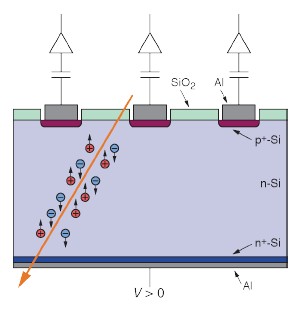
\includegraphics[width=0.5\textwidth]{immagini/rivelatore_a_semiconduttore.png}
\end{figure}
In tale schema la zona n rappresenta la parte principale della aggiunzione. Abbiamo poi dei contatti realizzati sopra con un $\rm p+$, e con un $\rm n+$ dall'altro lato.

Quando passa una particella all'interno della regione di svuotamento, essa deposita energia. Tale energia viene utilizzata per produrre coppie elettrone-lacuna, e queste coppie cominciano a migrare verso gli elettrodi per poi essere raccolte, in modo da indurre il segnale che andiamo poi a misurare. Lo schema è molto simile a quello che abbiamo visto per un rivelatore a gas, ciò che cambia è il mezzo in cui avviene il processo ed anche il tipo di processo, in quanto in tal caso produciamo coppie elettrone-lacuna mentre nel caso di un rivelatore a ionizzazione si producono coppie elettrone-ione. Ne approfittiamo per fare uno schema riassuntivo di quello che abbiamo visto finora nel campo della rivelazione:
\begin{figure}[H]
   \centering
   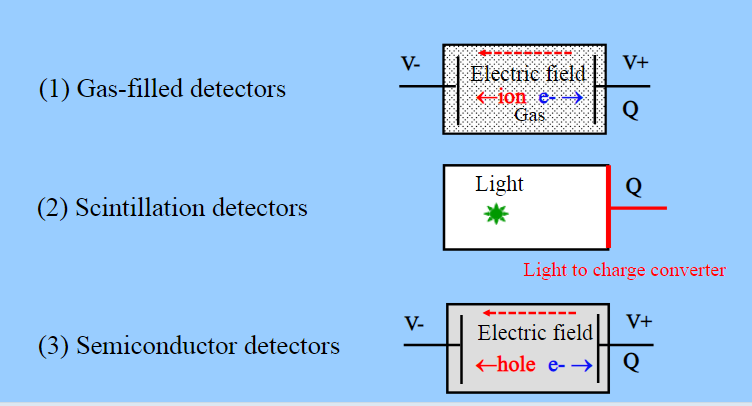
\includegraphics[width=0.7\textwidth]{immagini/schema_rivelatori.png}
\end{figure}
Vediamo come infatti i rivelatori a gas e i rivelatori a semiconduttore presentano uno schema molto similare, mentre i rivelatori a scintillazione hanno un comportamento diverso, in quanto si basano su principi fisici abbastanza diversi.

\vspace{0.2cm}Vediamo adesso come si realizza un rivelatore a semiconduttore, o meglio come si realizzano le giunzioni. Vengono utilizzati diversi processi per creare la barriera, noi vedremo quelli più utilizzati, che sono:

\begin{itemize}
   \item Rivelatori a diffusione;
   \item Rivelatori a barriera superficiale;
   \item Ion Implanted diodes;
   \item Rivelatori a deriva di Litio.
\end{itemize}

\subsection{Rivelatori a diffusione}
I rivelatori a diffusione vengono realizzati facendo diffondere delle impurità di tipo n (come ad esempio il fosforo) in un'estremità di un semiconduttore di tipo p. Per fare ciò sono necessarie delle elevate temperature, anche $1000 \; ^{\circ}\rm C$. Ottimizzando i tempi di diffusione e le concentrazioni si può ottenere una giunzione adeguata.
\begin{figure}[H]
   \centering
   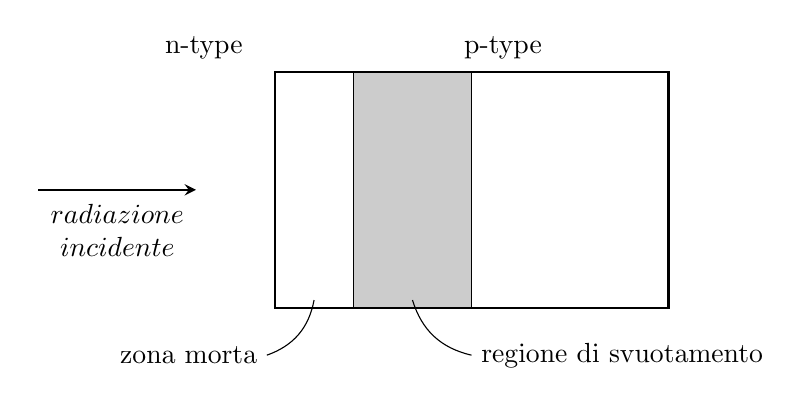
\begin{tikzpicture}
     \draw[fill=gray!40!] (1,-1.5) -- (1,1.5) -- (2.5,1.5) -- (2.5,-1.5) -- cycle;
      \draw[thick] (0,-1.5) -- (0,1.5) -- (5,1.5) -- (5,-1.5) -- cycle;
      \node at (-0.9,1.8) {n-type};
      \node at (2.9,1.8) {p-type};
      \draw[bend right] (-0.1,-2.1) node[left] {zona morta} to (0.5,-1.4);
      \draw[bend left] (2.5,-2.1) node[right] {regione di svuotamento} to (1.75,-1.4);
      \draw[thick,-stealth] (-3,0) -- (-1,0) node[midway,below]
      {$\begin{array}{c}
       \text{radiazione}\\
       \text{incidente}
       \end{array}$};
   \end{tikzpicture}
 \end{figure}
Tuttavia, il principale problema di questo tipo di rivelatori è che la giunzione non si forma in superficie, bensì si forma a una profondità di alcune decine di micron. Questo vuol dire che una particella che incide sul rivelatore dovrà attraversare prima una zona che per i nostri scopi è una zona morta, perché non è una zona utile per la rivelazione, per poi entrare nella regione di svuotamento. Ciò comporta una perdita dell'informazione trasportata dalla particella, il che limita le misure di energia. Tale fattore costituisce il principale svantaggio, inoltre un altro svantaggio sono le alte temperature che si adoperano, perché aumentano il rumore e tendono a diminuire la vita media dei portatori di carica, rendendo più difficile la loro misura. I vantaggi sono la robustezza e le basse contaminazioni superficiali.

\subsection{Rivelatori a barriera superficiale (SSB)}
Il problema della barriera a una certa profondità, dunque della presenza di una zona morta viene superato dai rivelatori a barriera superficiale. Questi sono basati su dei diodi Schottky, cioè dei diodi che si formano, anziché con due semiconduttore, con un semiconduttore e un metallo.
\begin{figure}[H]
   \centering
   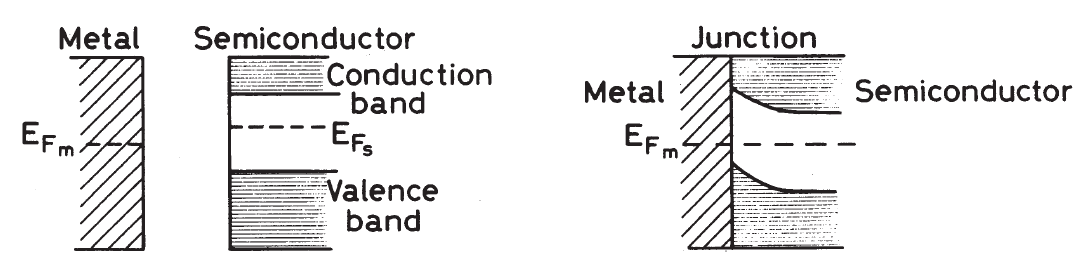
\includegraphics[width=0.9\textwidth]{immagini/rivelatori_a_barriera_superficiale.png}
\end{figure}
Quando infatti andiamo ad accostare un metallo con un semiconduttore, quello che succede è la formazione anche in questo caso di un aggiunzione. Solitamente si adopera dell'oro su un materiale di tipo n o dell'alluminio su un materiale di tipo p.

La produzione di questi rivelatori avviene innanzitutto trattando la superficie chimicamente, ossidandola e poi depositando lo strato metallico per evaporazione. Il tutto infine viene montato su un anello isolante con delle superfici metallizzate per assicurare il contatto elettrico.

\begin{minipage}{0.49\textwidth}
   \begin{figure}[H]
      \centering
      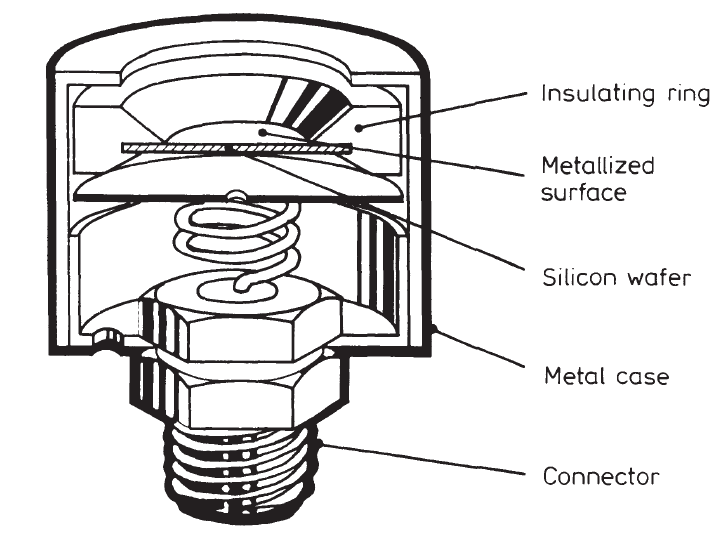
\includegraphics[width=0.9\textwidth]{immagini/schema_rivelatore_SSB.png}
   \end{figure}
\end{minipage}
\begin{minipage}{0.5\textwidth}
   \vspace{0.4cm}Il rivelatore che adoperiamo per l'esperienza della misura della radiazione $\alpha$ è di questa tipologia e si presenta così come mostrato nella figura accanto.
   
   L'esterno è l'anello su cui viene montato il tutto, mentre all'interno è posizionato il rivelatore che è una fetta di silicio. Il connettore ad avvitare permette infine il passaggio del segnale.
\end{minipage}

\vspace{0.3cm}Vediamo i vantaggi di questa tipologia di rivelatori:
\begin{itemize}[leftmargin=0.5cm]
   \item In questo caso abbiamo dei rivelatori totalmente svuotati, per cui non abbiamo nessuna zona morta come avveniva invece nel caso precedente;
   \item Possono essere profondi anche diversi millimetri. Nel nostro caso non ci interessa, però potrebbe essere utile per la rivelazione di altre particelle;
   \item Il processo di lavorazione avviene a temperatura ambiente, a differenza di quanto visto per i rivelatori a diffusione.
\end{itemize}
Per quanto riguarda gli svantaggi:
\begin{itemize}[leftmargin=0.5cm]
   \item Lo strato metallico depositato è così sottile che purtroppo non isola dalla luce, quindi sono rivelatori che possono essere sensibili alla luce. Infatti i fotoni del visibile hanno un'energia sufficiente a poter creare delle coppie elettrone-lacuna;
   \item Sono anche sensibili a possibili contaminazioni superficiali.
\end{itemize}

\subsection{Ion-Implanted Diodes}
Altre tipologie di rivelatori si basano invece sull'utilizzo dell'impiantazione ionica, in il drogaggio viene realizzato attraverso l'utilizzo di acceleratori che accelerano dei fasci di ioni, che sono le nostre impurità, per impiantarli all'interno di un materiale semiconduttore. \E un processo violento essendo sostanzialmente un bombardamento del materiale semiconduttore, e questo fa sì che alla fine sia necessario un annealing a $500 \, \rm ^{\circ}C$ per poter ripristinare i danni eventualmente causati da questo processo di impiantazione.

Per quanto riguarda i vantaggi, essi sono dei rivelatori molto stabili e con finestre di ingresso molto sottili, quindi con zona morta di poche decine di nanometri, ma lo svantaggio è che sono parecchio costosi, soprattutto per i processi di produzione che richiedono l'utilizzo di un acceleratore. 

\subsection{Rivelatori a deriva di litio Si(Li)}
L'ultima categoria di rivelatori che introduciamo sono i rivelatori a deriva di Litio, i quali cercano di risolvere il problema delle piccole dimensioni della regione di svuotamento, infatti abbiamo detto che c'è sempre un limite alle dimensioni di questa regione, perché poi il diodo va in rottura. Per risolvere questo problema si utilizza una cosiddetta aggiunzione p-i-n, dove al materiale di tipo p e al materiale di tipo n si frappone un materiale di tipo compensato. In questo modo è possibile ampliare la zona in cui può avvenire la rivelazione, potendo arrivare anche a spessori di $10-15$ mm, il che è molto utile laddove abbiamo bisogno di range elevati per poter fermare una particella e misurarne l'energia.

Vediamo il processo con cui avviene la realizzazione di questi rivelatori:
\begin{figure}[H]
   \centering
   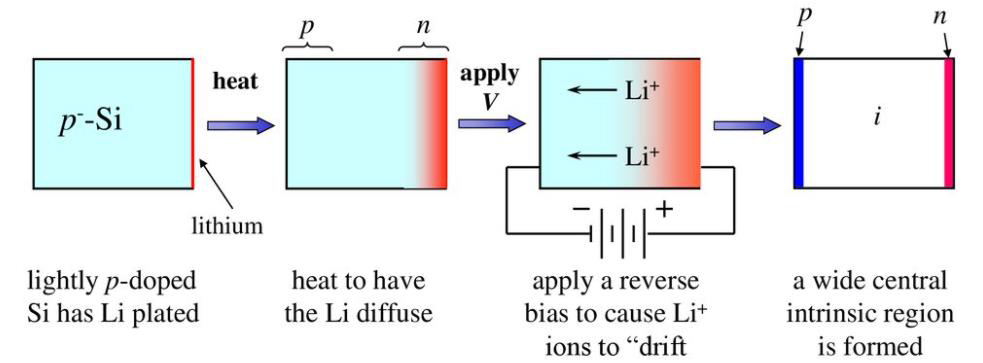
\includegraphics[width=\textwidth]{immagini/rivelatore_a_deriva_di_litio.png}
\end{figure}
Il litio viene posizionato sulla superficie di un materiale drogato di tipo p, viene fatto diffondere attraverso l'applicazione di un campo elettrico e alla fine quello che si ottiene è un'aggiunzione di tipo p-i-n, in quanto a sinistra rimane la zona p perché il litio non è arrivato fino a questa estremità, la regione centrale diventa di tipo compensato, perché era drogata di tipo p e ad essa aggiungiamo il litio che è di tipo n e infine a destra rimane la zona di tipo n dovuta essenzialmente a un'alta concentrazione di litio.

I vantaggi sono dovuti a questi spessori elevati, che fanno sì che vengano utilizzati per la spettroscopia beta o per i raggi X a bassa energia. Gli svantaggi sono invece il fatto che si debbano adoperare a temperature basse a causa dell'elevato rumore termico, inoltre anche la conservazione dovrebbe avvenire a temperatura basse per mantenere inalterata la zona intrinseca.

\subsection{Realizzazione contatti}
L'ultimo aspetto che discutiamo sul rivelatore al silicio riguarda la realizzazione dei contatti. 

Non è possibile creare un contatto ohmico utilizzando un materiale metallico sul semiconduttore perché quello che si viene a creare è un diodo Schottky, quindi un ulteriore giunzione e dunque un ulteriore regione di svuotamento, che non è ciò che desideriamo. Quello che allora si fa prima di applicare un contatto metallico è realizzare una regione altamente drogata, ad esempio nella figura seguente possiamo vedere una regione di tipo n+ prima del contatto metallico.
\begin{figure}[H]
   \centering
   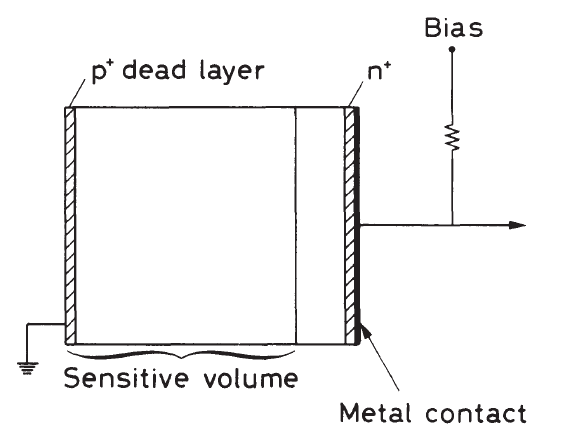
\includegraphics[width=0.5\textwidth]{immagini/realizzazione_contatti.png}
\end{figure}

\section{Caratteristiche dei rivelatori a semiconduttore}

\subsection{Linearità}
In ogni rivelatore che misura l'energia, ci aspettiamo un ottimo grado di linearità, per cui se arriva una particella con un'energia $E$ ci aspettiamo che il segnale prodotto sia proporzionale a tale energia, in maniera tale da avere una risposta lineare. Nel caso di un rivelatore a semiconduttore, se questo ha uno spessore sufficiente ad arrestare la particella al suo interno e quindi a misurare tutta l'energia, ci aspettiamo che il segnale in tensione che viene indotto sia proporzionale alla carica prodotta, quindi alle coppie elettrone-lacuna che sono state create a seguito della perdita di energia della particella all'interno del rivelatore, diviso la capacità, in quanto il diodo non è altro che un condensatore a causa della sua configurazione elettrica.

Se la radiazione ha energia $E$, allora dovrebbero essere create $E/w$ coppie elettrone-lacuna, dove $w$ è l'energia media per creare una coppia. In generale però il rivelatore avrà un'efficienza di raccolta $\eta$, che indica il fatto che non tutte le coppie prodotte potrebbero essere raccolte, dunque soltanto una carica $Q=\eta E/w$ e quindi il segnale misurato sarà dato da
\begin{equation*}
   V
   =\frac{Q}{C}
   =\eta \frac{E}{w C}
\end{equation*}
Il fatto che purtroppo perdiamo alcune coppie non ci spaventa, in quanto ciò che conta è che si mantenga la linearità tra il segnale prodotto e l'energia depositata nel rivelatore.

In generale, la risposta dei semiconduttori è abbastanza indipendente dal tipo di particella, quindi se entra un elettrone o se entra una particella alfa, normalmente se si deposita la stessa energia viene prodotto lo stesso segnale. Tale discorso è valido fintanto che non si considera l'arrivo di ioni: in tal caso di si generano degli effetti di plasma, quindi delle nuvole di elettroni particolarmente dense che vanno a distorcere il campo elettrico all'interno del rivelatore e pertanto la linearità non è del tutto assicurata.

Nel caso in cui invece il rivelatore non sia sufficientemente spesso, viene misurata semplicemente una perdita di energia, quindi a volte i rivelatori a semiconduttore vengono utilizzati come rivelatori di trasparenza, cioè con lo scopo di essere attraversati e far perdere alle particelle una quantità di energia molto piccola. In questo caso la risposta non è lineare con l'energia della particella.

\subsection{Risoluzione in energia}
La risoluzione di questi rivelatori è tipicamente abbastanza buona. Infatti servono pochi elettronVolt per generare una coppia elettrone-lacuna, a differenza dei valori di energia media per creare una coppia ione-elettrone in un rivelatore a gas che sono dell'ordine di $20-40$ eV. La conseguenza di ciò è che, a parità di energia depositata, nel caso di un rivelatore al silicio si produce un numero di coppie che è 10 volte superiore rispetto a quante se ne produrrebbero in un rivelatore a gas, e il fatto di avere un numero di coppie elevato fa sì che la risoluzione sia migliore.

\E chiaro che l'energia necessaria a creare una coppia dipende dal gap di energia proibita. Ad esempio, alla temperatura di 77 K per il silicio sono necessarie energie dell'ordine di $3-4$ eV letto, mentre per il germanio poco meno di 3 eV. Precisiamo che queste sono in realtà le energie per produrre una coppia, mentre le energie del gap sono in realtà più piccole. Ciò è legato al fatto che due terzi dell'energia vengono spesi per creare delle vibrazioni reticolari.

Prima di proseguire, facciamo alcune considerazioni. Quando vogliamo misurare l'energia, quest'ultima la misuriamo in termini del numero $n$ di coppie che si generano. Tale numero è dato dal rapporto tra l'energia $E$ che viene depositata nel rivelatore diviso $w$, che è l'energia media per creare una coppia. Ciò vale sia per i rivelatori a gas che per i rivelatori a semiconduttore, con l'unica differenza che nei rivelatori a gas $w$ è dell'ordine all'incirca di 30 eV mentre nel rivelatore a semiconduttore $w$ è dell'ordine di circa 3 eV, quindi circa un decimo. Più precisamente il numero di coppie a cui facciamo riferimento è un valore medio $\bar{n}$, perché sebbene sia vero che si produce un certo numero di coppie quelle che poi danno luogo al segnale sono una parte poiché avvengono diversi fenomeni di fluttuazioni statistiche. Ne segue che il numero $\bar{n}$ che misuriamo e che è indice dell'energia in realtà può variare da evento a evento. Immaginiamo ad esempio, come facciamo in un'esperienza di laboratorio, di inviare in un rivelatore al silicio delle particelle $\alpha$ di 5 MeV. Tale energia viene totalmente depositata nel rivelatore, dando luogo a un certo numero di coppie che produrranno il segnale, e questo numero di coppie fluttuerà a seguito di fenomeni di natura statistica.

Se andiamo a misurare lo spettro in energia delle particelle $\alpha$, dato che l'energia è legata al numero di coppie generate, a tale picco ne corrisponderà uno relativo al numero di queste:

\begin{figure}[H]
   \centering
   \begin{tikzpicture}
      %assi
      \draw[->] (-3,0) -- (3.5,0) node[right] {$n$};
      \draw[->] (-3,0) -- (-3,4.5) node[above] {$N_{\alpha}$};
      %grafico
      \draw[red!60!black,thick] plot[domain=-3:3, smooth] (\x,{4*exp(-3*(\x)^2)});
      \draw (0,0.1) -- (0,-0.1) node[below] {$\bar{n}$};
      %FWHM
      \draw[<->] (-0.4806,2) -- (0.4806,2);
      \begin{scope}[shift={(-8cm, 0cm)}]
         %assi
         \draw[->] (-3,0) -- (3.5,0) node[right] {$E$};
         \draw[->] (-3,0) -- (-3,4.5) node[above] {$N_{\alpha}$};
         %grafico
         \draw[red!60!black,thick] plot[domain=-3:3, smooth] (\x,{4*exp(-(\x)^2)});
         %FWHM
         \draw[<->] (-0.832,2) -- (0.832,2) node[midway, below] {\footnotesize FWHM};
      \end{scope}
    \end{tikzpicture}
\end{figure}

Quello che osserviamo è un picco molto stretto, il quale rappresenta il numero di particelle $\alpha$ che hanno una certa energia. Il fatto di non avere una delta di Dirac come ci aspetteremmo, dato che stiamo inviando particelle di 5 MeV e quindi in teoria dovremmo trovare sempre lo stesso valore, è dovuto al fatto che ci sono delle fluttuazioni nel numero di coppie che creano il segnale, quindi quello che osserviamo nello spettro in energia è una conseguenza del numero di coppie $n$ che ogni volta si producono e che vengono raccolte, il quale non è sempre lo stesso. In sintesi abbiamo un valore medio $\bar{n}$ dato $\bar{n}=E/w$ e rispetto a questo ogni volta abbiamo delle fluttuazioni.

La risoluzione in energia $R$ viene valutata andando a guardare il picco e studiandone la larghezza, in particolare ci concentriamo sulla larghezza a metà altezza FWHM, a cui la risoluzione è legata mediante la relazione
\begin{equation*}
   R=\frac{\rm FWHM}{E}
\end{equation*}
Se il picco ha una forma gaussiana si può dimostrare che la FWHM è all'incirca $2.35 \sigma$, dove $\sigma$ è la deviazione standard della gaussiana.

Vediamo adesso come mettere in relazione la risoluzione al numero di coppie. Scrivendo l'energia in termini del numero medio di coppie prodotte abbiamo $E=\bar{n}W$, per quanto riguarda invece la deviazione standard della distribuzione in energie, essa è legata alla deviazione standard della distribuzione del numero di coppie mediante la relazione $\sigma_E=w \sigma_n$. Andando a sostituire la risoluzione in energia diventa
\begin{equation*}
   R
   =\frac{2.35w \sigma_n}{\bar{n} w}
   =2.35\frac{\sigma_n}{n}
\end{equation*}
In definitiva la risoluzione sarà dato dalla larghezza della distribuzione del numero di coppie sul numero medio di coppia generato. Se la distribuzione che regola la produzione di queste coppie è di tipo Poissoniano, possiamo approssimare $\sigma$ con $\sqrt{n}$ e riscrivere ulteriormente la risoluzione come
\begin{equation*}
   R=\frac{2.35}{\sqrt{n}}
\end{equation*}
Per quanto detto prima, a parità di energia in un rivelatore a silicio si producono un numero di coppie pari a 10 volte il numero che se ne producono in un rivelatore a gas, per cui avremo che $R_{\rm Si}=R_{\rm gas}/\sqrt{10}$, per cui è circa un terzo più piccola e dunque migliore.
Nei rivelatori al silicio si possono raggiungere anche risoluzioni dell'1\%

\subsection{Sensibilità ed efficienza intrinseca}

L'efficienza intrinseca di un rivelatore a semiconduttore è dell'ordina del 100\%. Ricordiamo che l'efficienza intrinseca rappresenta il rapporto tra il numero di particelle che hanno dato luogo a un segnale diviso il numero di particelle incidenti, in quanto in generale non è detto che una particella incide sul rivelatore perdendo energia sia in grado di produrre un segnale rivelabile, mentre in questo caso sì.

Tali rivelatori presentano dei limiti. Uno di questi è la presenza di una soglia minima necessaria sul segnale da rivelare, legata al fatto che ci sono delle correnti di dispersione e che l'elettronica introduce un minimo di rumore. Tali fattori possono creare dei segnali di rumore, i quali hanno bassa ampiezza, dunque per non confonderli con segnali fisici dobbiamo in qualche modo discriminarli, cioè eliminarli dell'acquisizione. Questo può essere fatto imponendo una soglia minima al di sotto della quale non acquisire nulla. Tale soglia da un lato ci aiuta a eliminare il rumore, dall'altro però potrebbe far perdere qualche segnale fisico di interesse, quindi abbassare leggermente l'efficienza intrinseca. Allo stesso modo, la presenza di una zona morta potrebbe imporre una certa perdita nell'efficienza perché magari particelle di bassa energia non riescono ad attraversare tale zona e quindi non vengono misurate, quindi hanno inciso sul rivelatore ma non sono state misurate.

\subsection{Densità}
L'elevata densità di tali rivelatori costituisce un vantaggio perché permette di avere un elevato stopping power, il che ci permette di avere rivelatori compatti ma comunque capaci di misurare l'energia di particelle anche molto energetiche.

\begin{esempio}
   Nel seguente grafico è riportata l'energia della particella nell'intervallo tra 1 e 100 MeV e sulle ordinate il range in micron. Le varie linee corrispondono a diverse tipologie di particelle che incidono sul silicio.

   \begin{minipage}{0.39\textwidth}
      \begin{figure}[H]
         \centering
         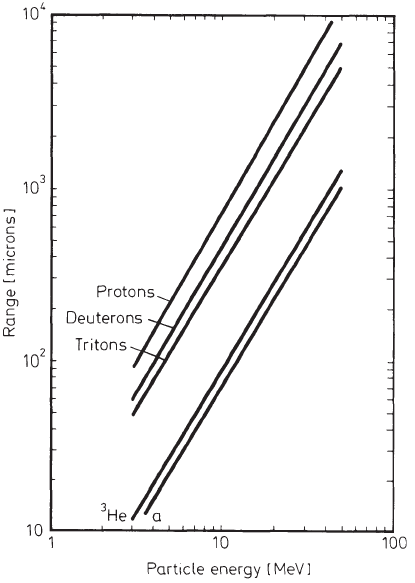
\includegraphics[width=\textwidth]{immagini/range_particelle_in_semiconduttori.png}
      \end{figure}
   \end{minipage}
   \begin{minipage}{0.6\textwidth}
      A partire da tale grafico possiamo capire che spessore deve avere il rivelatore per assicurarci che tutta l'energia venga persa all'interno del rivelatore. Ad esempio per particelle $\alpha$ da 5 MeV come quelle che adoperiamo in laboratorio servono range dell'ordine della ventina di micron, quindi è sufficiente un rivelatore di questo spessore per far sì che le particelle $\alpha$ perdano tutta la loro energia. Infine, un'ultima qualità di questi rivelatori che abbiamo una diffusione estremamente più bassa, più piccola rispetto a quelle rivelatori a gas, si fa sì che questi rivelatori possono essere utilizzati più facilmente come rivelatori di posizione, quindi per andare a misurare la posizione della particelle incidente.
   \end{minipage}
\end{esempio}

Infine un'ultima qualità di questi rivelatori è che abbiamo una diffusione estremamente più bassa rispetto a quelle rivelatori a gas, e ciò si fa sì che questi rivelatori possano essere utilizzati più facilmente come rivelatori di posizione, cioè per misurare la posizione della particelle incidente.

\subsection{Tempo di risposta}

Sono rivelatori molto veloci. In generale possono essere utilizzati come rivelatori di timing molto più performanti rispetto ai classici rivelatori a gas. Tipicamente i tempi di salita di un segnale sono dell'ordine dei nanosecondi, quindi estremamente veloci.

\subsection{Danneggiamento da radiazione}
Un problema di questi rivelatori è il cosiddetto danneggiamento da radiazione, che si verifica se questi rivelatori vengono esposti a notevoli dosi di radiazione. Purtroppo ciò avviene soprattutto in alcuni ambienti come gli esperimenti sotto fascio o esperimenti nello spazio e ciò modifica le qualità e le proprietà del rivelatore.

In generale i danni che si possono creare sono di due diversi tipi:
\begin{itemize}
   \item Danni del Bulk, cioè danni della massa che costituisce il semiconduttore;
   \item Danni sulla superficie, quindi sull'ossido che normalmente riveste questi rivelatori.
\end{itemize}

Gli effetti sul bulk sono effetti che si manifestano come danneggiamento al reticolo e in generale sono dovuti alle cosiddette radiazioni non ionizzanti, in inglese NIEL (Non Ionizing Energy Loss). Esse possono comportare
\begin{itemize}[leftmargin=0.5cm]
   \item Un cambio della tensione di svuotamento, che comporta uno svuotamento minore e quindi la necessità di applicare tensioni maggiori;
   \item Un aumento della corrente di leakage\footnote{La corrente di leakage (in italiano, corrente di dispersione) è una piccola corrente elettrica che scorre attraverso un percorso indesiderato o inatteso, solitamente dovuto a fenomeni come l'imperfezione dell'isolamento o perdite tra i conduttori di un circuito elettrico e il suolo o altre parti del sistema.}, che è una corrente che comporta un rumore il quale potrebbe richiedere l'utilizzo di un raffreddamento;Danni sulla superficie, quindi sull'ossido che normalmente riveste questi rivelatori.
   \item Una diminuzione nell'efficienza nella raccolta della carica.
\end{itemize}

%Lo studio dei possibili danneggiamenti da radiazione è una parte importante nella progettazione di un esperimento. Ad esempio tutti gli esperimenti acceleratori come può essere l'HCO o altri acceleratori richiedono anni e anni di progettazione anche per studiare questi effetti. Perché sono arrivelatori che ovviamente richiedono lo sforzo di anni di lavoro e devono operare per almeno 5, 10 anni. quindi bisogna assicurarsi che il rivalatore non subnisca un deterioramento eccessivo e che quindi possa lavorare per l'intervallo di tempo in cui dovrebbe lavorare. Quindi spesso la tecnologia non esiste nel momento in cui si immagina di dover costruire il rivalatore, quindi si lavora per costruire e arrivare a questi obiettivi.

Gli effetti sulla superficie sono invece tipicamente dovuti a radiazione ionizzante e questo comporta sostanzialmente la presenza di cariche positive che si accumulano sugli ossidi e poi può anche influire sul rumore e sulla tensione di rottura.

Gli effetti che vengono prodotti dal danneggiamento da radiazione possono essere
\begin{itemize}[leftmargin=0.5cm]
   \item Effetti cumulativi, che si vanno sommando nel tempo e sono dei danni che non si possono riparare, dovuti all'esposizione prolungata alla radiazione come nel caso di un rivelatore adoperato in un esperimento sotto fascio;
   \item Eventi singoli che possono essere o eventi transitori o eventi catastrofici permanenti. Siccome possono accadere in qualsiasi istante, non sono legati ad un accumulo a differenza del caso precedente.
\end{itemize}

\comment{\section{Applicazioni nella spettroscopia di particelle cariche}
A causa della loro risposta temporale abbastanza veloce e della loro ottima risoluzione, i rivelatori a semiconduttore vengono utilizzati nel campo della spettroscopia di particelle cariche.

Inoltre sono disponibili in un'ampia varietà sia di spessori che anche di area sensibile, hanno un'efficienza prossima al 100\% nel caso di protoni, particelle alfa ma anche ioni pesanti e di ricevo che lo spessore da adoperare chiaramente si deve valutare in base all'applicazione, quindi in base al tipo di particella che si vuole andare a parlare in base anche alla sua energia. E proprio per questo motivo nel campo della fisica moderna, più che fisica moderna della fisica attuale, soprattutto fisica delle alte energie, questi rivelatori vengono utilizzati ampiamente, hanno appunto le prestazioni proprio adatte per andare ad affrontare anche degli ambienti spavorevoli, come ambienti in cui si ha una elevata dose di radiazione, una elevata densità di particelle e quindi negli ultimi decenni ci sono stati enormi sviluppi soprattutto in questo campo con ovviamente ritadute poi in altre tipologie di applicazioni come ad esempio il campo della medicina, quindi tante volte alcune tecnologie si sviluppano nel campo della ricerca e poi vengono trasferite in automatico nel campo, in altri tipi di campo, campo arespaziale, campo della medicina. Un altro vantaggio di questi rivelatori è che spesso è utile avere dei rivelatori molto subtili, vi ho detto che questi rivelatori possono essere adoperati anche come rivelatori in trasparenza, vengono attraversati della particella, viene effettivamente depositata dell'energia, ma questa energia è molto piccola, quindi è come se fosse una piccola perturbazione effettivamente del percorso e della particella nelle sue proprietà. E questo è un vantaggio perché da un lato abbiamo comunque sia un segnale che mi indica il fatto che è passato una particella e quindi eventualmente per problematiche di tracciamento di tracking, quindi sapere attraverso quali punti la particella è passata è utile avere questi rivelatori perché sono in grado proprio di misurare la posizione della particella senza perturbarne eccessivamente le caratteristiche. Quindi ormai tutti, quasi tutti gli esperimenti di alta energia e nello spazio utilizzano ampiamente questi rivelatori al silicio. Questo è un grafico che ormai è un po' datato perché insomma risale ormai quasi a vent'anni fa, però era giusto per darvi un'idea vent'anni fa di quali erano gli esperimenti che tipicamente utilizzavano rivelatori in questo caso al silicio di tecnologia strip, ora vi dirò un po' qualcosa qualcosa questa tecnologia. Comunque al di là di questo dettaglio vedete colorati le diverse applicazioni, questi sono acceleratori, quindi quindi verde e rosso si riferiscono a esperimenti prestoacceleratori e l'HC è l'acceleratore al momento più potente che riesce ad accelerare alle massime energie fino a la realizzata mentre in blu vengono riportati gli esperimenti nello spazio. Quindi vedete che appunto... ma che è questo rumore ragazzi? Sto riuscendo a favori. Ansì rispetto a qualche giorno fa, a qualche qualche di giorni fa. A inizio febbraio abbiamo fatto un esame del dottorato, un esame fino a il dottorato qui in quest'aula, è stato un inferno veramente, non si capiva niente. Comunque, vi dicevo, vedete appunto la varietà di applicazioni qui sotto sono riportati proprio nel dettaglio le sigle degli esperimenti che fanno uso di questa tecnologia al siri. Cioè, ad esempio, quello che mostra la maggiora utilizza, ad esempio l'esperimento CMS, non so se l'abbiamo mai seguito nominare, un esperimento presso l'acceleratore e l'HC. Diciamo uno dei esperimenti che ha contribuita alla scoperta del bosone X. E vedete qui il grafico riporta l'area in metri quadri. Quindi Quindi questo caso, vedete, CMS utilizza 214 metri quadri di rivelatori, in questo caso al siriscio in strippo. Ma altri rivelatori non sono da meno, comunque una tecnologia particolarmente utilizzata.}

\section{Tipologie moderne di rivelatori al silicio}
Guardiamo ora più più dettaglio alcuni rivelatori più moderni che utilizzano la tecnologia basata sul silicio, in particolare ne sfruttano le buone capacità di tracciamento (cioè la risoluzione spaziale) e la risoluzione energetica.

\begin{minipage}{0.39\textwidth}
   \begin{figure}[H]
      \centering
      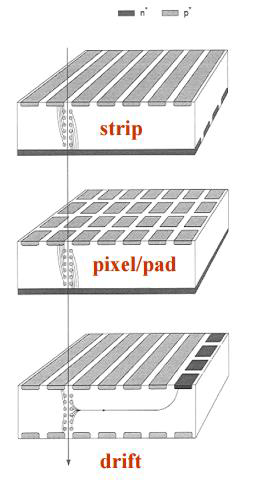
\includegraphics[width=\textwidth]{immagini/Tipi_rivelatore_al_silicio.png}
   \end{figure}
\end{minipage}
\begin{minipage}{0.6\textwidth}
   Quando si vuole utilizzare il silicio per ricostruire la posizione della particella che incide sul rivelatore, si hanno due possibili scelte:
   \begin{itemize}[leftmargin=0.5cm]
      \item readout continuo
      \item readout discreto
   \end{itemize}
   Nel seguito discuteremo la differenza tra i due e in particolare approfondiremo i rivelatori a strip e quelli a pixel o pad per quanto concerne il readout discreto e quelli a drift per quanto concerne il readout continuo. Possiamo vedete un'immediata differenza nella rappresentazione accanto: il rivelatore a strip presenta delle strisce parallele, dette appunto strip in inglese, di materiale semiconduttore; il rivelatore a pixel o pad, presenta una matrice di elementi che prendono proprio il nome di pixel; infine quelli a drift presentano nuovamente una struttura a strisce, però come vedremo c'è qualche differenza rispetto al caso delle strip.
\end{minipage}

\subsection{Rivelatori a strip}
I primi rivelatori che approfondiamo sono quelli a strip o microstrip nel caso in cui le strip abbiano dimensioni di pochi micron. Vediamo la struttura di questo rivelatore:
\begin{figure}[H]
   \centering
   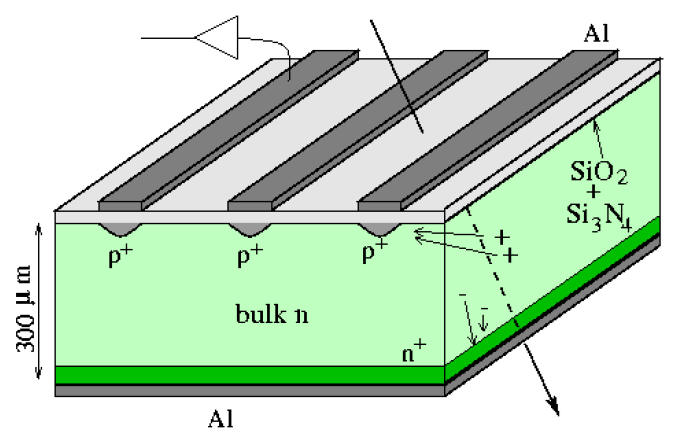
\includegraphics[width=0.5\textwidth]{immagini/rivelatori_a_strip.png}
\end{figure}
Il principio di funzionamento si basa ancora su giunzioni p-n, però in più si sfrutta il fatto di poter realizzare gli elettrodi con determinate geometrie. In questo caso gli elettrodi di lettura sono costituiti da delle strip che vengono posizionate parallelamente l'un l'altra ad una distanza opportuna tipicamente della decina di micron. Il segnale che viene prodotto all'interno del rivelatore induce il segnale sull'elettrodo sull'elettrodo più vicino. Quindi quando una particella attraversa il rivelatore, questa produrrà un certo numero di coppie elettrone-lacuna che migreranno verso gli elettrodi, inducendo un segnale, \E chiaro che la strip che viene interessata ci fornirà la coordinata spaziale, cioè il punto attraverso cui è passata la particella. Si tratta di un'informazione monodimensionale, perché l'unica informazione che abbiamo nel piano è lungo la direzione perpendicolare alle strip. Per ottenere un'informazione bidimensionale sul piano, una tecnica che viene adoperata è consiste nel sovrapporre due strati di rivelatore a strip con una certa inclinazione tra loro, come possiamo vedere nella seguente figura:
\begin{figure}[H]
   \centering
   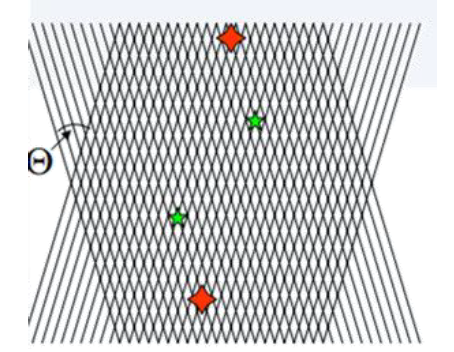
\includegraphics[width=0.4\textwidth]{immagini/angolo_rivelatore_a_strip.png}
\end{figure}
Così facendo conosciamo le strip interessate su ciascun piano, ottenendo così l'informazione bidimensionale.

Tale tecnica può però portare a dei casi di ambiguità: se passa una sola particella attraverso entrambi gli strati allora non c'è alcuna ambiguità perché verrà interessata una strip per piano, ma se per caso sono più particelle ad attraversare simultaneamente i due strati come può avvenire ad esempio in un esperimento sotto fascio, allora inevitabilmente si crea un'ambiguità.

Guardando la figura dei due strati di strip, vediamo che è raffigurata la situazione in cui sono passate due particelle simultaneamente. Ciascuno strato avrà due strip interessate (una per particella), quindi nel momento in cui vogliamo risalire alla posizione dovremo considerare quattro possibili combinazioni di queste coppie di strip. I due punti verdi rappresentano le combinazioni corrette, cioè i punti reali attraverso cui sono passate le particelle, mentre i punti rossi rappresentano delle combinazioni spurie, in quanto non collegate al reale passaggio di particelle. 

La risoluzione spaziale, cioè la precisione con cui si ricostruisce la posizione dipende dalla distanza tra le strip: più queste sono vicino tra di loro, migliore sarà la risoluzione spaziale. Similmente alle camere a fili, data la distanza tra due elettrodi la risoluzione è data da tale distanza $\sqrt{12}$, che è una conseguenza del teorema del limite centrale. Si tratta quindi di una risoluzione molto spinta, potendo arrivare anche a 5 micron.

I tempi di raccolta delle cariche sono molto veloci, anche decine di nanosecondi.

Il rivelatore a strip è un esempio di rivelatore a redout discreto, perché qui la posizione viene data grazie alla discretizzazione dell'elettrodo, cioè al fatto di avere tanti elettrodi separati.

\subsection{Rivelatori a drift}

In un rivelatore ad drift invece abbiamo un redout continuo. Rispetto a prima il rivelatore a drift fornisce entrambe le coordinate su un piano, quindi un'informazione bidimensionale.
\begin{figure}[H]
   \centering
   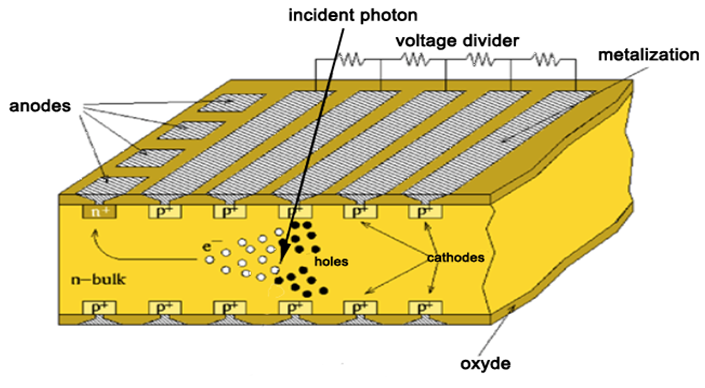
\includegraphics[width=0.6\textwidth]{immagini/rivelatori_a_drift.png}
\end{figure}
La struttura sembra molto simile a quella strip. VAbbiamo sempre degli elettrodi che sono realizzati come strip paralleli l'un all'altro, ma questi in realtà hanno una funzione diversa rispetto a quella che abbiamo visto prima. Ciò che raccoglie il segnale sono in realtà degli anodi sotto forma di pad, cioè di piazzola.

Quando passa una particella in grado di produrre coppie elettrone-lacuna, gli elettroni prodotti cominciano a migrare verso gli anodi grazie a una differenza di potenziale che viene realizzata attraverso le strip, le quali vengono messe a potenziale via via crescente in maniera tale che gli elettroni vengano guidati verso l'anodo.

Vediamo come facciamo ad avere la coordinata bidimensionale. La coordinata lungo l'asse parallelo alla direzione delle strip viene fornita da quale anodo è stato interessato, cioè quello che ha raccolto la carica; l'altra coordinata, cioè quella nella direzione perpendicolare alle strip che è anche quella lungo cui si muovono gli elettroni, viene fornita dal tempo di deriva, cioè da quanto tempo impiegano gli elettroni ad arrivare all'anodo, che chiaramente dipende dal punto in cui si sono prodotti. 

Lo svantaggio di questi rivelatori è che essi sono più lenti perché bisogna aspettare una deriva degli elettroniche può essere anche abbastanza lunga e inoltre necessitano di temperature stabili.

Il rivelatore a drift costituisce un esempio di rivelatore al readout continuo, perché sebbene sia vero che lungo la direzione parallela alle strip abbiamo una discretizzazione dovuta agli anodi, lungo l'altra direzione la lettura è continua, cioè il tempo di deriva assume un valore che non è discreto bensì continuo.

\subsection{CCD (Charged-Coupled-Device)}
Un altro dispositivo molto simile a quello appena visto è il CCD, cioè il Charged Couple Device, il quale è l'elemento di base delle fotocamere. Anche questi CCD sono rivelatori al readout continuo, si dicono anche rivelatori a memoria perché gli elettroni che vengono prodotti a seguito della ionizzazione non sono rimossi immediatamente, quindi non vengono raccolti immediatamente da un elettrodo, ma vengono innanzitutto confinati all'interno di un pixel e poi a poco a poco vengono fatti derivare fino alla raccolta finale.
\begin{figure}[H]
   \centering
   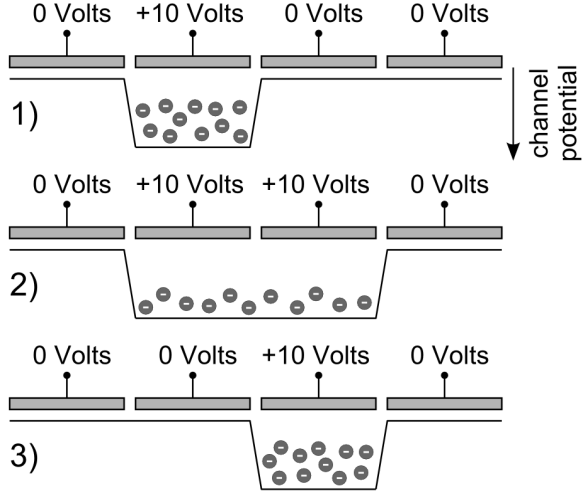
\includegraphics[width=0.6\textwidth]{immagini/CCD.png}
\end{figure}
Il CCD è costituito da una matrice di pixel, che costituiscono righe e colonne. Quando questo sensore viene attraversato dalla luce, viene generata della carica e questa carica non viene raccolta immediatamente da un elettrodo, bensì a seconda del punto in cui si è creata viene guidata lungo la colonna corrispondente. Supponiamo ad esempio, come in figura, che la carica sia stata prodotta nel secondo pixel. Allora, grazie a un campo elettrico opportuno, quindi a delle differenze di potenziale, è possibile guidare la carica prodotta da pixel a pixel fino ad arrivare all'ultima riga dove avviene la lettura. Quello che succede è che via via viene creato un potenziale positivo nel pixel adiacente a dove si trova la carica e azzerato nel precedente, il che permette la deriva delle cariche. Grazie a questo sistema è possibile risalire a quale pixel è interessato.

I CCD sono rivelatori bidimensionali, cioè ci forniscono la posizione in cui è avvenuta la rivelazione, hanno accuratezze spaziali anche molto elevate, dell'ordine di 10 micron, però hanno come difetto principale un tempo di lettura molto lungo, dell'ordine di 10 millisecondi. Ciò fa sì che questi rivelatori non possono essere adoperati nel campo della fisica delle alte energie perché sono troppo lenti. In un esperimento in un acceleratore avvengono un certo numero di collisioni al secondo, per cui se il rivelatore fosse ancora impegnato a misurare ciò che è avvenuto nell'evento precedente, succederebbe il cosiddetto pile up, cioè una sovrapposizione di eventi che è chiaramente da evitare. Tuttavia tali rivelatori vengono adoperati parecchio nel campo dell'astronomia, n particolare avendo una bassa risoluzione energetica e spaziale vengono utilizzati per spettroscopia di raggi X.

\subsection{Rivelatori a pixel}

Funzionano in maniera analoga i cosiddetti rivelatori a pixel, i quali vengono adoperati nel campo della fisica nucleare e che sono molto più veloci rispetto ai CCD.

I rivelatori a pixel sono anch'essi costituiti da matrici di pixel che, a seconda della superficie da rivestire, possono essere anche dell'ordine di centinaia di milioni di pixel complessivamente, i quali però sono dei canali indipendenti, dunque ritorniamo a un caso di readout discreto perché è come se ogni pixel fosse un rivelatore indipendente dall'altro. La risoluzione spaziale del rivelatore dipende dalle dimensioni di questi pixel, in particolare sarà migliore al diminuire delle dimensioni, che ormai possono arrivare anche a $15-20 \, \rm \mu m$ per lato. Sono ovviamente rivelatori bidimensionali perché viene fornita sia la coordinata $x$ che la coordinata $y$.

Sono inoltre rivelatori che hanno un livello di rumore molto basso, il che dipende dalla bassa capacità elettrica di questi rivelatori, quindi hanno un buon rapporto segnale su rumore $S/N$. Ciò vuol dire che quando vengono attraversati da una radiazione si produce una carica e quindi un segnale che si sopraeleva rispetto al fondo. Sono rivelatori veloci e sono particolarmente adatti nel caso di alte densità di particelle, in quanto la probabilità che due particelle cadano in un pixel di dimensioni così piccole è veramente bassa. Ecco perché questi rivelatori normalmente vengono posizionati nella regione a più alta densità, quindi ad esempio in un collider, dove avviene un'interazione tra due fasci uno contro l'altro, vengono adoperati nella zona più vicina al punto di collisione, che è quella con la densità di particelle più elevata, mentre allontanandoci diventa sempre meno necessario avere rivelatori così discreti

Gli svantaggi di tali rivelatori è che abbiamo un numero di canali enorme da leggere, e siccome in linea di principio ogni rivelatore ha bisogno di un connettore e di un cavo la situazione diventa particolarmente ostica, soprattutto considerando il fatto che dobbiamo adoperare cavi di dimensioni ridotte.
\begin{figure}[H]
   \centering
   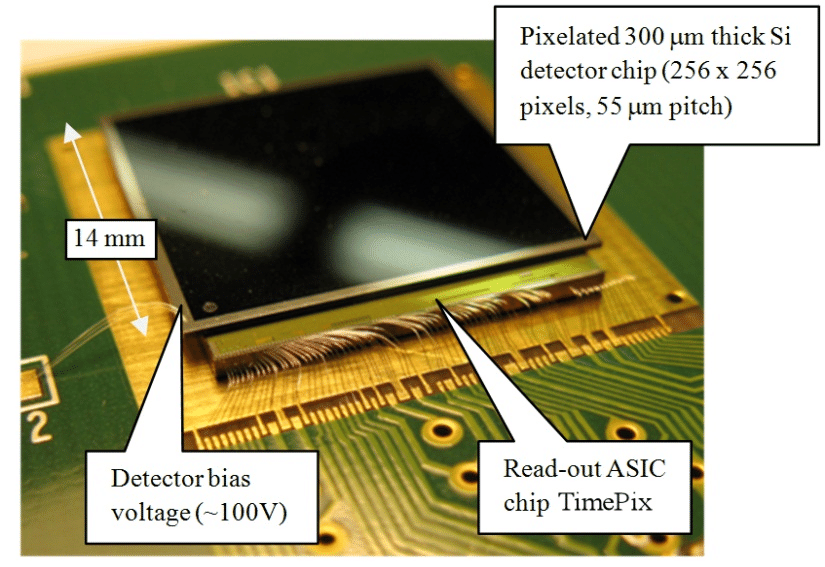
\includegraphics[width=0.6\textwidth]{immagini/zoom_rivelatore_silicio.png}
\end{figure}
In figura possiamo vedere un ingrandimento di quello che è un rivelatore a pixel. Guardando attentamente, vediamo che ci sono dei fili microscopici che sono detti bonding, cioè delle connessioni che vengono realizzate con delle opportune macchine chiamate bondatrici, le quali collegano il rivelatore con l'elettronica.

Inoltre questi rivelatori sono molto fragili e richiedono tecnologia all'avanguardia. Vediamo il motivo di quest'ultimo fatto. Innanzitutto il primo problema è quello di trasportare questo segnale fuori da ciascun pixel che è un rivelatore a sé stante, quindi se il segnale che fuoriesce da questo rivelatore ha bisogno di un'opportuna catena elettronica, questa dovrà essere replicata per tutti i pixel. Quello che si faceva tempo addietro (ora questa è una tecnologia che si sta superando) era realizzare l'elettronica miniaturizzata e delle stesse dimensioni dei pixel.

\begin{figure}[H]
   \centering
   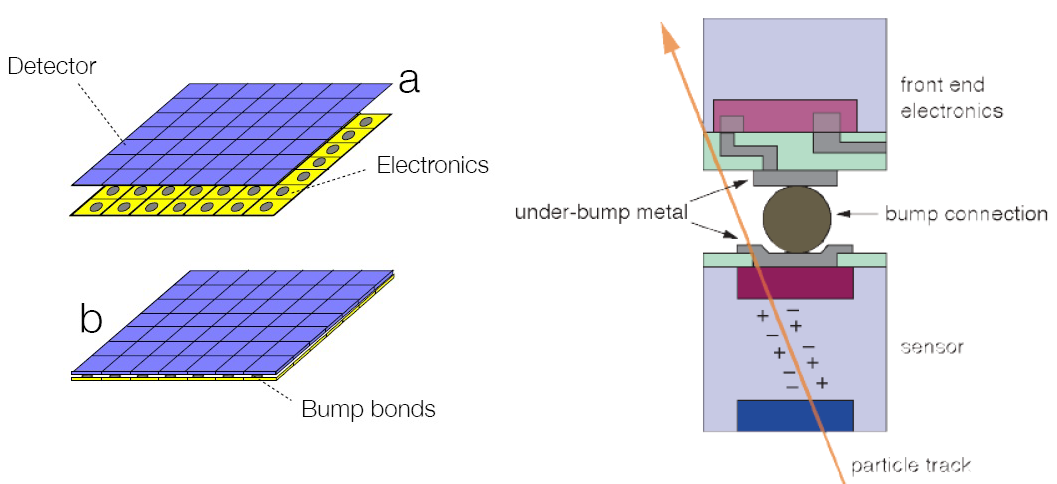
\includegraphics[width=\textwidth]{immagini/connessione_rivelatore_a_pixel.png}
\end{figure}

Si aveva quindi una matrice di pixel che erano i rivelatori e sotto una matrice con la corrispondente elettronica. La connessione si realizzava attraverso una tecnica che prende il nome di bump bonding, cioè un bonding non realizzato con un filo, bensì con una pallina di materiale conduttore, come possiamo vedere in figura a destra. Chiaramente la corrispondenza tra pixel di sensore e pixel di elettronica deve essere esatta. Il tutto avviene a temperatura controllata, perché la pallina si deve sciogliere per realizzare un contatto stabile.

Tuttavia questa tecnica aveva dei difetti enormi, in particolare un'efficienza estremamente bassa e presentavano frequentemente dei difetti, quindi spesso si buttavano tanti wafer di silicio perché il bonding non era stato realizzato bene. Inoltre era un processo molto costoso e che limita la dimensione del pixel, quindi anche se la tecnologia ci permetteva di ridurre le dimensioni del pixel, l'elettronica non si riusciva a compattare al di sotto di un certo limite e anche il bonding non poteva essere effettuato su pixel di dimensioni troppo piccole. Inoltre, sempre nell'ottica di rendere il rivelatore il più possibile trasparente, inserire una pallina di un qualsiasi materiale introduce ovviamente una perdita di energia dato che la particella dovrà attraversare anche questa, la quale può rappresentare anche un problema di multiple scattering. 

Adesso la tecnologia ci permette di realizzare i così detti MAPS (Monolithic Active Pixel Sensors), cioè rivelatori monolitici. Con tale termine si intende il fatto che nello stesso substrato di silicio si realizza sia il sensore che l'elettronica.
\begin{figure}[H]
   \centering
   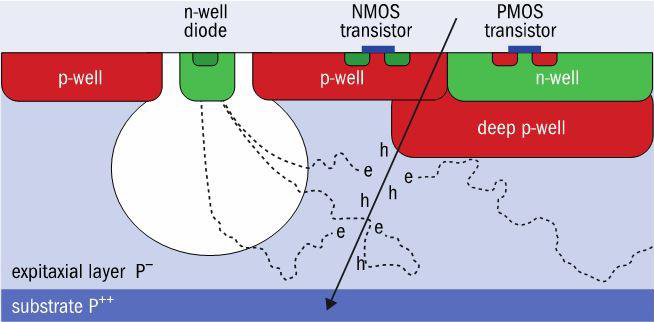
\includegraphics[width=0.7\textwidth]{immagini/rivelatore_monolitico.png}
\end{figure}
Ne segue che non abbiamo più bisogno del bonding, quindi guadagniamo in termini di efficienza. Tuttavia il problema iniziale di questa tecnologia era il fatto che essa era poco resistente alla radiazione, quindi perdeva in prestazioni man mano che si accumulava la dose. Ormai questi limiti sono stati superati, quindi questa tecnologia viene utilizzata in tantissimi esperimenti.